\documentclass[twoside]{book}

% Packages required by doxygen
\usepackage{fixltx2e}
\usepackage{calc}
\usepackage{doxygen}
\usepackage[export]{adjustbox} % also loads graphicx
\usepackage{graphicx}
\usepackage[utf8]{inputenc}
\usepackage{makeidx}
\usepackage{multicol}
\usepackage{multirow}
\PassOptionsToPackage{warn}{textcomp}
\usepackage{textcomp}
\usepackage[nointegrals]{wasysym}
\usepackage[table]{xcolor}

% NLS support packages
\usepackage[catalan]{babel}

% Font selection
\usepackage[T1]{fontenc}
\usepackage[scaled=.90]{helvet}
\usepackage{courier}
\usepackage{amssymb}
\usepackage{sectsty}
\renewcommand{\familydefault}{\sfdefault}
\allsectionsfont{%
  \fontseries{bc}\selectfont%
  \color{darkgray}%
}
\renewcommand{\DoxyLabelFont}{%
  \fontseries{bc}\selectfont%
  \color{darkgray}%
}
\newcommand{\+}{\discretionary{\mbox{\scriptsize$\hookleftarrow$}}{}{}}

% Page & text layout
\usepackage{geometry}
\geometry{%
  a4paper,%
  top=2.5cm,%
  bottom=2.5cm,%
  left=2.5cm,%
  right=2.5cm%
}
\tolerance=750
\hfuzz=15pt
\hbadness=750
\setlength{\emergencystretch}{15pt}
\setlength{\parindent}{0cm}
\setlength{\parskip}{3ex plus 2ex minus 2ex}
\makeatletter
\renewcommand{\paragraph}{%
  \@startsection{paragraph}{4}{0ex}{-1.0ex}{1.0ex}{%
    \normalfont\normalsize\bfseries\SS@parafont%
  }%
}
\renewcommand{\subparagraph}{%
  \@startsection{subparagraph}{5}{0ex}{-1.0ex}{1.0ex}{%
    \normalfont\normalsize\bfseries\SS@subparafont%
  }%
}
\makeatother

% Headers & footers
\usepackage{fancyhdr}
\pagestyle{fancyplain}
\fancyhead[LE]{\fancyplain{}{\bfseries\thepage}}
\fancyhead[CE]{\fancyplain{}{}}
\fancyhead[RE]{\fancyplain{}{\bfseries\leftmark}}
\fancyhead[LO]{\fancyplain{}{\bfseries\rightmark}}
\fancyhead[CO]{\fancyplain{}{}}
\fancyhead[RO]{\fancyplain{}{\bfseries\thepage}}
\fancyfoot[LE]{\fancyplain{}{}}
\fancyfoot[CE]{\fancyplain{}{}}
\fancyfoot[RE]{\fancyplain{}{\bfseries\scriptsize Generat per Doxygen }}
\fancyfoot[LO]{\fancyplain{}{\bfseries\scriptsize Generat per Doxygen }}
\fancyfoot[CO]{\fancyplain{}{}}
\fancyfoot[RO]{\fancyplain{}{}}
\renewcommand{\footrulewidth}{0.4pt}
\renewcommand{\chaptermark}[1]{%
  \markboth{#1}{}%
}
\renewcommand{\sectionmark}[1]{%
  \markright{\thesection\ #1}%
}

% Indices & bibliography
\usepackage{natbib}
\usepackage[titles]{tocloft}
\setcounter{tocdepth}{3}
\setcounter{secnumdepth}{5}
\makeindex

% Hyperlinks (required, but should be loaded last)
\usepackage{ifpdf}
\ifpdf
  \usepackage[pdftex,pagebackref=true]{hyperref}
\else
  \usepackage[ps2pdf,pagebackref=true]{hyperref}
\fi
\hypersetup{%
  colorlinks=true,%
  linkcolor=blue,%
  citecolor=blue,%
  unicode%
}

% Custom commands
\newcommand{\clearemptydoublepage}{%
  \newpage{\pagestyle{empty}\cleardoublepage}%
}

\usepackage{caption}
\captionsetup{labelsep=space,justification=centering,font={bf},singlelinecheck=off,skip=4pt,position=top}

%===== C O N T E N T S =====

\begin{document}

% Titlepage & ToC
\hypersetup{pageanchor=false,
             bookmarksnumbered=true,
             pdfencoding=unicode
            }
\pagenumbering{alph}
\begin{titlepage}
\vspace*{7cm}
\begin{center}%
{\Large Pràctica (Primavera 2020) \\[1ex]\large Ricard Guixaró Trancho }\\
\vspace*{1cm}
{\large Generat per Doxygen 1.8.13}\\
\end{center}
\end{titlepage}
\clearemptydoublepage
\pagenumbering{roman}
\tableofcontents
\clearemptydoublepage
\pagenumbering{arabic}
\hypersetup{pageanchor=true}

%--- Begin generated contents ---
\chapter{Pràctica (Primavera 2020).}
\label{index}\hypertarget{index}{}En esta practica se construye un programa modular que ofrece un menú de opciones para gestionar un almacen. Se introducen las clases {\itshape \hyperlink{class_cjt__productos}{Cjt\+\_\+productos}}, {\itshape \hyperlink{class_sala}{Sala}}, {\itshape \hyperlink{class_cjt__salas}{Cjt\+\_\+salas}} y {\itshape \hyperlink{class_almacen}{Almacen}}. 
\chapter{Índex de Classes}
\section{Llista de Classes}
Aquestes són les classes, estructures, unions i interfícies acompanyades amb breus descripcions\+:\begin{DoxyCompactList}
\item\contentsline{section}{\hyperlink{class_cjt__estudiants}{Cjt\+\_\+estudiants} \\*Representa un conjunt d\textquotesingle{}estudiants ordenat per D\+NI }{\pageref{class_cjt__estudiants}}{}
\item\contentsline{section}{\hyperlink{class_estudiant}{Estudiant} \\*Representa un estudiant amb D\+NI i la possibilitat de tenir nota }{\pageref{class_estudiant}}{}
\end{DoxyCompactList}

\chapter{Índex de Fitxers}
\section{Llista dels Fitxers}
Aquesta és la llista de tots els fitxers acompanyats amb breus descripcions\+:\begin{DoxyCompactList}
\item\contentsline{section}{\hyperlink{_bin_tree_8hh}{Bin\+Tree.\+hh} }{\pageref{_bin_tree_8hh}}{}
\item\contentsline{section}{\hyperlink{_cjt___clusters_8cc}{Cjt\+\_\+\+Clusters.\+cc} \\*Implementació de la classe \hyperlink{class_cjt___clusters}{Cjt\+\_\+\+Clusters} }{\pageref{_cjt___clusters_8cc}}{}
\item\contentsline{section}{\hyperlink{_cjt___clusters_8hh}{Cjt\+\_\+\+Clusters.\+hh} \\*Especificació de la classe \hyperlink{class_cjt___clusters}{Cjt\+\_\+\+Clusters} }{\pageref{_cjt___clusters_8hh}}{}
\item\contentsline{section}{\hyperlink{_cjt___especies_8cc}{Cjt\+\_\+\+Especies.\+cc} \\*Implementació de la classe \hyperlink{class_cjt___especies}{Cjt\+\_\+\+Especies} }{\pageref{_cjt___especies_8cc}}{}
\item\contentsline{section}{\hyperlink{_cjt___especies_8hh}{Cjt\+\_\+\+Especies.\+hh} \\*Especificació de la classe \hyperlink{class_cjt___especies}{Cjt\+\_\+\+Especies} }{\pageref{_cjt___especies_8hh}}{}
\item\contentsline{section}{\hyperlink{_cluster_8cc}{Cluster.\+cc} \\*Implementació de la classe \hyperlink{class_cluster}{Cluster} }{\pageref{_cluster_8cc}}{}
\item\contentsline{section}{\hyperlink{_cluster_8hh}{Cluster.\+hh} \\*Especificació de la classe \hyperlink{class_cluster}{Cluster} }{\pageref{_cluster_8hh}}{}
\item\contentsline{section}{\hyperlink{_especie_8cc}{Especie.\+cc} \\*Implementació de la classe \hyperlink{class_especie}{Especie} }{\pageref{_especie_8cc}}{}
\item\contentsline{section}{\hyperlink{_especie_8hh}{Especie.\+hh} \\*Especificació de la classe \hyperlink{class_especie}{Especie} }{\pageref{_especie_8hh}}{}
\item\contentsline{section}{\hyperlink{program_8cc}{program.\+cc} \\*Programa principal de la pràctica }{\pageref{program_8cc}}{}
\end{DoxyCompactList}

\chapter{Documentació de les Classes}
\hypertarget{class_cjt___clusters}{}\section{Referència de la Classe Cjt\+\_\+\+Clusters}
\label{class_cjt___clusters}\index{Cjt\+\_\+\+Clusters@{Cjt\+\_\+\+Clusters}}


Representa un conjunt de clusters.  


\subsection*{Mètodes públics}
\begin{DoxyCompactItemize}
\item 
\hyperlink{class_cjt___clusters_a2e55759944a78043744103e19dd87c1c}{Cjt\+\_\+\+Clusters} ()
\begin{DoxyCompactList}\small\item\em Creadora per defecte. \end{DoxyCompactList}\item 
void \hyperlink{class_cjt___clusters_ace64164c455de6b3e91b774ad95d93ac}{add\+\_\+cluster} (const \hyperlink{class_cluster}{Cluster} \&A, string id)
\begin{DoxyCompactList}\small\item\em Afegir un cluster a un conjunt. \end{DoxyCompactList}\item 
void \hyperlink{class_cjt___clusters_a779452d093c92ec42e47987a84ea48ff}{erase\+\_\+cluster} (\hyperlink{class_cluster}{Cluster} A)
\begin{DoxyCompactList}\small\item\em Esborrar un cluster d\textquotesingle{}un conjunt. \end{DoxyCompactList}\item 
void \hyperlink{class_cjt___clusters_a35d2c4c28bee51017f4ac9049a0fe6e9}{initialize\+\_\+clusters} (\hyperlink{class_cjt___especies}{Cjt\+\_\+\+Especies} \&A)
\begin{DoxyCompactList}\small\item\em Inicialitza un conjunt de clusters. \end{DoxyCompactList}\item 
void \hyperlink{class_cjt___clusters_ac2bf2811c291533e3516ad4de8240d36}{wpgma\+\_\+algorithm} ()
\begin{DoxyCompactList}\small\item\em Executa l\textquotesingle{}algorisme W\+P\+G\+MA. \end{DoxyCompactList}\item 
double \hyperlink{class_cjt___clusters_acd0e381a6b4c43933b3c6761febf9b3e}{cluster\+\_\+distance} (\hyperlink{class_cluster}{Cluster} A, \hyperlink{class_cluster}{Cluster} B)
\begin{DoxyCompactList}\small\item\em Consultora de la distància entre dos clusters. \end{DoxyCompactList}\item 
void \hyperlink{class_cjt___clusters_ad794d3d1b0df7adb7fbb35d21634f5a0}{clusters\+\_\+distance\+\_\+update} (bool indicador, string id)
\begin{DoxyCompactList}\small\item\em Actualiza l\textquotesingle{}element table\+\_\+clusters d\textquotesingle{}un conjunt. \end{DoxyCompactList}\item 
pair$<$ string, string $>$ \hyperlink{class_cjt___clusters_a3db57ec9903b4f5439679ac9ba41fab1}{dmin} (double \&x)
\begin{DoxyCompactList}\small\item\em Consultora dels clusters a menor distància. \end{DoxyCompactList}\item 
bool \hyperlink{class_cjt___clusters_aaa57cbd8d86567b4403ac9adb34a87f5}{cluster\+\_\+exist} (string id)
\begin{DoxyCompactList}\small\item\em Consultora de l\textquotesingle{}existència d\textquotesingle{}un cluster al conjunt. \end{DoxyCompactList}\item 
int \hyperlink{class_cjt___clusters_a1ecfc9a82c3a0dff467769880c355efd}{clusters\+\_\+set\+\_\+size} () const
\begin{DoxyCompactList}\small\item\em Consultora de la mida d\textquotesingle{}un conjunt. \end{DoxyCompactList}\item 
void \hyperlink{class_cjt___clusters_af0dffae314624bb0ab6f6c7f8e28a770}{print\+\_\+final\+\_\+cluster} ()
\begin{DoxyCompactList}\small\item\em Escriptura del primer/últim cluster d\textquotesingle{}un conjunt. \end{DoxyCompactList}\item 
void \hyperlink{class_cjt___clusters_a0072a1e21a58e0ab64ac96ccff068229}{find\+\_\+print\+\_\+cluster} (string id)
\begin{DoxyCompactList}\small\item\em Escriptura del cluster al qual pertany l\textquotesingle{}id. \end{DoxyCompactList}\item 
void \hyperlink{class_cjt___clusters_acc4dd33e82c36c394acd44e60f77da22}{print\+\_\+table\+\_\+clusters} ()
\begin{DoxyCompactList}\small\item\em Escriptura de table\+\_\+clusters. \end{DoxyCompactList}\end{DoxyCompactItemize}
\subsection*{Tipus Privats}
\begin{DoxyCompactItemize}
\item 
typedef map$<$ string, \hyperlink{class_cluster}{Cluster} $>$\+::const\+\_\+iterator \hyperlink{class_cjt___clusters_ad9cf46a8e1e6430c7b34b184f2756054}{mclu\+\_\+iterator}
\item 
typedef map$<$ string, double $>$\+::const\+\_\+iterator \hyperlink{class_cjt___clusters_abdef6142bd4683a878bb393a9095555e}{table\+\_\+clusters\+\_\+column\+\_\+iterator}
\begin{DoxyCompactList}\small\item\em Typedef d\textquotesingle{}un iterator que recorre una columna (map$<$string, double$>$) d\textquotesingle{}una taula de clusters. \end{DoxyCompactList}\item 
typedef map$<$ string, map$<$ string, double $>$ $>$\+::const\+\_\+iterator \hyperlink{class_cjt___clusters_ac53ace59de6ecf75f90d7a4fc6e56c0e}{table\+\_\+clusters\+\_\+iterator}
\begin{DoxyCompactList}\small\item\em Typedef d\textquotesingle{}un iterator que recorre una taula de clusters (map$<$string, map$<$string, double$>$$>$) \end{DoxyCompactList}\end{DoxyCompactItemize}
\subsection*{Atributs Privats}
\begin{DoxyCompactItemize}
\item 
map$<$ string, \hyperlink{class_cluster}{Cluster} $>$ \hyperlink{class_cjt___clusters_a5f5e13255bca1fac2ad65c51473f6ead}{mclu}
\begin{DoxyCompactList}\small\item\em Map que emmagatzema els clusters del conjunt. \end{DoxyCompactList}\item 
map$<$ string, map$<$ string, double $>$ $>$ \hyperlink{class_cjt___clusters_a6af3fcf70683cdb88f137f6f51002939}{table\+\_\+clusters}
\begin{DoxyCompactList}\small\item\em Matriu de les distancies entre els clusters del conjunt. \end{DoxyCompactList}\end{DoxyCompactItemize}


\subsection{Descripció Detallada}
Representa un conjunt de clusters. 

Definició a la línia 20 del fitxer Cjt\+\_\+\+Clusters.\+hh.



\subsection{Documentació de les Definicions de Tipus Membre}
\mbox{\Hypertarget{class_cjt___clusters_ad9cf46a8e1e6430c7b34b184f2756054}\label{class_cjt___clusters_ad9cf46a8e1e6430c7b34b184f2756054}} 
\index{Cjt\+\_\+\+Clusters@{Cjt\+\_\+\+Clusters}!mclu\+\_\+iterator@{mclu\+\_\+iterator}}
\index{mclu\+\_\+iterator@{mclu\+\_\+iterator}!Cjt\+\_\+\+Clusters@{Cjt\+\_\+\+Clusters}}
\subsubsection{\texorpdfstring{mclu\+\_\+iterator}{mclu\_iterator}}
{\footnotesize\ttfamily typedef map$<$string, \hyperlink{class_cluster}{Cluster}$>$\+::const\+\_\+iterator \hyperlink{class_cjt___clusters_ad9cf46a8e1e6430c7b34b184f2756054}{Cjt\+\_\+\+Clusters\+::mclu\+\_\+iterator}\hspace{0.3cm}{\ttfamily [private]}}



Definició a la línia 25 del fitxer Cjt\+\_\+\+Clusters.\+hh.

\mbox{\Hypertarget{class_cjt___clusters_abdef6142bd4683a878bb393a9095555e}\label{class_cjt___clusters_abdef6142bd4683a878bb393a9095555e}} 
\index{Cjt\+\_\+\+Clusters@{Cjt\+\_\+\+Clusters}!table\+\_\+clusters\+\_\+column\+\_\+iterator@{table\+\_\+clusters\+\_\+column\+\_\+iterator}}
\index{table\+\_\+clusters\+\_\+column\+\_\+iterator@{table\+\_\+clusters\+\_\+column\+\_\+iterator}!Cjt\+\_\+\+Clusters@{Cjt\+\_\+\+Clusters}}
\subsubsection{\texorpdfstring{table\+\_\+clusters\+\_\+column\+\_\+iterator}{table\_clusters\_column\_iterator}}
{\footnotesize\ttfamily typedef map$<$string, double$>$\+::const\+\_\+iterator \hyperlink{class_cjt___clusters_abdef6142bd4683a878bb393a9095555e}{Cjt\+\_\+\+Clusters\+::table\+\_\+clusters\+\_\+column\+\_\+iterator}\hspace{0.3cm}{\ttfamily [private]}}



Typedef d\textquotesingle{}un iterator que recorre una columna (map$<$string, double$>$) d\textquotesingle{}una taula de clusters. 



Definició a la línia 31 del fitxer Cjt\+\_\+\+Clusters.\+hh.

\mbox{\Hypertarget{class_cjt___clusters_ac53ace59de6ecf75f90d7a4fc6e56c0e}\label{class_cjt___clusters_ac53ace59de6ecf75f90d7a4fc6e56c0e}} 
\index{Cjt\+\_\+\+Clusters@{Cjt\+\_\+\+Clusters}!table\+\_\+clusters\+\_\+iterator@{table\+\_\+clusters\+\_\+iterator}}
\index{table\+\_\+clusters\+\_\+iterator@{table\+\_\+clusters\+\_\+iterator}!Cjt\+\_\+\+Clusters@{Cjt\+\_\+\+Clusters}}
\subsubsection{\texorpdfstring{table\+\_\+clusters\+\_\+iterator}{table\_clusters\_iterator}}
{\footnotesize\ttfamily typedef map$<$string, map$<$string, double$>$ $>$\+::const\+\_\+iterator \hyperlink{class_cjt___clusters_ac53ace59de6ecf75f90d7a4fc6e56c0e}{Cjt\+\_\+\+Clusters\+::table\+\_\+clusters\+\_\+iterator}\hspace{0.3cm}{\ttfamily [private]}}



Typedef d\textquotesingle{}un iterator que recorre una taula de clusters (map$<$string, map$<$string, double$>$$>$) 



Definició a la línia 33 del fitxer Cjt\+\_\+\+Clusters.\+hh.



\subsection{Documentació del Constructor i el Destructor}
\mbox{\Hypertarget{class_cjt___clusters_a2e55759944a78043744103e19dd87c1c}\label{class_cjt___clusters_a2e55759944a78043744103e19dd87c1c}} 
\index{Cjt\+\_\+\+Clusters@{Cjt\+\_\+\+Clusters}!Cjt\+\_\+\+Clusters@{Cjt\+\_\+\+Clusters}}
\index{Cjt\+\_\+\+Clusters@{Cjt\+\_\+\+Clusters}!Cjt\+\_\+\+Clusters@{Cjt\+\_\+\+Clusters}}
\subsubsection{\texorpdfstring{Cjt\+\_\+\+Clusters()}{Cjt\_Clusters()}}
{\footnotesize\ttfamily Cjt\+\_\+\+Clusters\+::\+Cjt\+\_\+\+Clusters (\begin{DoxyParamCaption}{ }\end{DoxyParamCaption})}



Creadora per defecte. 

S\textquotesingle{}executa automàticament al declarar un \hyperlink{class_cjt___clusters}{Cjt\+\_\+\+Clusters}.

\begin{DoxyPrecond}{Precondició}
{\itshape cert} 
\end{DoxyPrecond}
\begin{DoxyPostcond}{Postcondició}
Crea un conjunt de clusters. 
\end{DoxyPostcond}


Definició a la línia 9 del fitxer Cjt\+\_\+\+Clusters.\+cc.


\begin{DoxyCode}
9                            \{
10 \}
\end{DoxyCode}


\subsection{Documentació de les Funcions Membre}
\mbox{\Hypertarget{class_cjt___clusters_ace64164c455de6b3e91b774ad95d93ac}\label{class_cjt___clusters_ace64164c455de6b3e91b774ad95d93ac}} 
\index{Cjt\+\_\+\+Clusters@{Cjt\+\_\+\+Clusters}!add\+\_\+cluster@{add\+\_\+cluster}}
\index{add\+\_\+cluster@{add\+\_\+cluster}!Cjt\+\_\+\+Clusters@{Cjt\+\_\+\+Clusters}}
\subsubsection{\texorpdfstring{add\+\_\+cluster()}{add\_cluster()}}
{\footnotesize\ttfamily void Cjt\+\_\+\+Clusters\+::add\+\_\+cluster (\begin{DoxyParamCaption}\item[{const \hyperlink{class_cluster}{Cluster} \&}]{A,  }\item[{string}]{id }\end{DoxyParamCaption})}



Afegir un cluster a un conjunt. 

Afegeix el cluster del paràmetre al conjunt de clusters del paràmetre implícit i actualiza table\+\_\+clusters afegint on sigui necessari la distància amb el nou cluster.

\begin{DoxyPrecond}{Precondició}
El cluster no pertany al conjunt del paràmetre implícit. 
\end{DoxyPrecond}
\begin{DoxyPostcond}{Postcondició}
Afegeix el cluster al conjunt del paràmetre implícit i actualiza table. 
\end{DoxyPostcond}


Definició a la línia 14 del fitxer Cjt\+\_\+\+Clusters.\+cc.


\begin{DoxyCode}
14                                                           \{
15     \hyperlink{class_cjt___clusters_a5f5e13255bca1fac2ad65c51473f6ead}{mclu}.insert(make\_pair(\textcolor{keywordtype}{id}, A));
16     \textcolor{keywordtype}{bool} indicador = \textcolor{keyword}{true};
17     \hyperlink{class_cjt___clusters_ad794d3d1b0df7adb7fbb35d21634f5a0}{clusters\_distance\_update}(indicador, \textcolor{keywordtype}{id});
18 \}   
\end{DoxyCode}
\mbox{\Hypertarget{class_cjt___clusters_a779452d093c92ec42e47987a84ea48ff}\label{class_cjt___clusters_a779452d093c92ec42e47987a84ea48ff}} 
\index{Cjt\+\_\+\+Clusters@{Cjt\+\_\+\+Clusters}!erase\+\_\+cluster@{erase\+\_\+cluster}}
\index{erase\+\_\+cluster@{erase\+\_\+cluster}!Cjt\+\_\+\+Clusters@{Cjt\+\_\+\+Clusters}}
\subsubsection{\texorpdfstring{erase\+\_\+cluster()}{erase\_cluster()}}
{\footnotesize\ttfamily void Cjt\+\_\+\+Clusters\+::erase\+\_\+cluster (\begin{DoxyParamCaption}\item[{\hyperlink{class_cluster}{Cluster}}]{A }\end{DoxyParamCaption})}



Esborrar un cluster d\textquotesingle{}un conjunt. 

Elimina el cluster del paràmetre del conjunt de clusters del paràmetre implícit i actualiza table\+\_\+clusters suprimint qualsevol presència del cluster eliminat.

\begin{DoxyPrecond}{Precondició}
El cluster pertany al conjunt del paràmetre implícit. 
\end{DoxyPrecond}
\begin{DoxyPostcond}{Postcondició}
Elimina el cluster del conjunt del paràmetre implícit i actualiza table. 
\end{DoxyPostcond}


Definició a la línia 20 del fitxer Cjt\+\_\+\+Clusters.\+cc.


\begin{DoxyCode}
20                                           \{
21     \textcolor{keywordtype}{string} \textcolor{keywordtype}{id} = A.\hyperlink{class_cluster_a7e077596f7eb4f2bdf2847d65fa37654}{query\_cluster\_id}();
22     \hyperlink{class_cjt___clusters_a5f5e13255bca1fac2ad65c51473f6ead}{mclu}.erase(\textcolor{keywordtype}{id});
23     \hyperlink{class_cjt___clusters_a6af3fcf70683cdb88f137f6f51002939}{table\_clusters}.erase(\textcolor{keywordtype}{id});
24     \textcolor{keywordtype}{bool} indicador = \textcolor{keyword}{false};
25     \hyperlink{class_cjt___clusters_ad794d3d1b0df7adb7fbb35d21634f5a0}{clusters\_distance\_update}(indicador, \textcolor{keywordtype}{id});
26 \}
\end{DoxyCode}
\mbox{\Hypertarget{class_cjt___clusters_a35d2c4c28bee51017f4ac9049a0fe6e9}\label{class_cjt___clusters_a35d2c4c28bee51017f4ac9049a0fe6e9}} 
\index{Cjt\+\_\+\+Clusters@{Cjt\+\_\+\+Clusters}!initialize\+\_\+clusters@{initialize\+\_\+clusters}}
\index{initialize\+\_\+clusters@{initialize\+\_\+clusters}!Cjt\+\_\+\+Clusters@{Cjt\+\_\+\+Clusters}}
\subsubsection{\texorpdfstring{initialize\+\_\+clusters()}{initialize\_clusters()}}
{\footnotesize\ttfamily void Cjt\+\_\+\+Clusters\+::initialize\+\_\+clusters (\begin{DoxyParamCaption}\item[{\hyperlink{class_cjt___especies}{Cjt\+\_\+\+Especies} \&}]{A }\end{DoxyParamCaption})}



Inicialitza un conjunt de clusters. 

Primer de tot, buida el map de clusters (mclu) i la matriu de distàncies (table\+\_\+clusters). Inicialitza el conjunt de clusters amb el conjunt d\textquotesingle{}espècies del paràmetre i table\+\_\+clusters amb table\+\_\+species.

\begin{DoxyPrecond}{Precondició}
{\itshape cert} 
\end{DoxyPrecond}
\begin{DoxyPostcond}{Postcondició}
Inicialitza el conjunt de clusters amb el conjunt d\textquotesingle{}espècies i table\+\_\+clusters amb table\+\_\+species. 
\end{DoxyPostcond}


Definició a la línia 28 del fitxer Cjt\+\_\+\+Clusters.\+cc.


\begin{DoxyCode}
28                                                       \{
29     \textcolor{keywordflow}{if} (\hyperlink{class_cjt___clusters_a5f5e13255bca1fac2ad65c51473f6ead}{mclu}.size() != 0) \{
30         \hyperlink{class_cjt___clusters_a5f5e13255bca1fac2ad65c51473f6ead}{mclu}.erase(\hyperlink{class_cjt___clusters_a5f5e13255bca1fac2ad65c51473f6ead}{mclu}.begin(), \hyperlink{class_cjt___clusters_a5f5e13255bca1fac2ad65c51473f6ead}{mclu}.end());
31         \hyperlink{class_cjt___clusters_a6af3fcf70683cdb88f137f6f51002939}{table\_clusters}.erase(\hyperlink{class_cjt___clusters_a6af3fcf70683cdb88f137f6f51002939}{table\_clusters}.begin(), 
      \hyperlink{class_cjt___clusters_a6af3fcf70683cdb88f137f6f51002939}{table\_clusters}.end());
32     \}
33     \textcolor{keywordtype}{int} i = 0;
34     \textcolor{keywordflow}{while} (i < A.\hyperlink{class_cjt___especies_a011e96e195dfe5997d42e7937fe2099c}{species\_set\_size}()) \{
35         \textcolor{keywordtype}{string} \textcolor{keywordtype}{id} = A.\hyperlink{class_cjt___especies_af33bf6763e518251a77642136064bdbf}{returnid}(i);
36         \hyperlink{class_cluster}{Cluster} a(\textcolor{keywordtype}{id}, 0);
37         \hyperlink{class_cjt___clusters_a5f5e13255bca1fac2ad65c51473f6ead}{mclu}.insert(make\_pair(\textcolor{keywordtype}{id}, a));
38         ++i;
39     \}
40     \textcolor{keywordflow}{for} (\hyperlink{class_cjt___clusters_ad9cf46a8e1e6430c7b34b184f2756054}{mclu\_iterator} it = \hyperlink{class_cjt___clusters_a5f5e13255bca1fac2ad65c51473f6ead}{mclu}.begin(); it != \hyperlink{class_cjt___clusters_a5f5e13255bca1fac2ad65c51473f6ead}{mclu}.end(); ++it) \{
41         map<string, double> aux;
42         \textcolor{keywordtype}{double} x = 0;
43         \textcolor{keywordflow}{for} (\hyperlink{class_cjt___clusters_ad9cf46a8e1e6430c7b34b184f2756054}{mclu\_iterator} it1 = it; it1 != \hyperlink{class_cjt___clusters_a5f5e13255bca1fac2ad65c51473f6ead}{mclu}.end(); ++it1) \{
44             \textcolor{keywordflow}{if} (it->first != it1->first) \{
45                 x = A.\hyperlink{class_cjt___especies_ae13d0a3a9f8b0ed9bba78b1c6c9d4eaa}{returndist}(it->first, it1->first);
46                 aux.insert(make\_pair(it1->first, x));
47             \}
48         \}
49         \hyperlink{class_cjt___clusters_a6af3fcf70683cdb88f137f6f51002939}{table\_clusters}.insert(make\_pair(it->first, aux));
50     \}
51 \}
\end{DoxyCode}
\mbox{\Hypertarget{class_cjt___clusters_ac2bf2811c291533e3516ad4de8240d36}\label{class_cjt___clusters_ac2bf2811c291533e3516ad4de8240d36}} 
\index{Cjt\+\_\+\+Clusters@{Cjt\+\_\+\+Clusters}!wpgma\+\_\+algorithm@{wpgma\+\_\+algorithm}}
\index{wpgma\+\_\+algorithm@{wpgma\+\_\+algorithm}!Cjt\+\_\+\+Clusters@{Cjt\+\_\+\+Clusters}}
\subsubsection{\texorpdfstring{wpgma\+\_\+algorithm()}{wpgma\_algorithm()}}
{\footnotesize\ttfamily void Cjt\+\_\+\+Clusters\+::wpgma\+\_\+algorithm (\begin{DoxyParamCaption}{ }\end{DoxyParamCaption})}



Executa l\textquotesingle{}algorisme W\+P\+G\+MA. 

Fusiona els dos clusters a menor distància i els elimina del conjunt. Afegeix el cluster fusionat al conjunt i afegeix un pair$<$string, double$>$ a distancies amb l\textquotesingle{}identificador concatenat i la distància a la qual es trobaven els dos clusters.

\begin{DoxyPrecond}{Precondició}
La mida del conjunt de clusters del paràmetre implícit és $>$ 1. 
\end{DoxyPrecond}
\begin{DoxyPostcond}{Postcondició}
Fusiona en un nou cluster els dos clusters que es troben a menor distància, i els elimina del conjunt. Afegeix al conjunt el cluster resultant i es guarda la distància entre els dos clusters fusionats i l\textquotesingle{}identificador a l\textquotesingle{}atribut distancies. 
\end{DoxyPostcond}


Definició a la línia 53 del fitxer Cjt\+\_\+\+Clusters.\+cc.


\begin{DoxyCode}
53                                    \{
54     \textcolor{keywordtype}{double} x;
55     pair<string, string> u = \hyperlink{class_cjt___clusters_a3db57ec9903b4f5439679ac9ba41fab1}{dmin}(x);
56     \hyperlink{class_cjt___clusters_ad9cf46a8e1e6430c7b34b184f2756054}{mclu\_iterator} it1 = \hyperlink{class_cjt___clusters_a5f5e13255bca1fac2ad65c51473f6ead}{mclu}.find(u.first);
57     \hyperlink{class_cjt___clusters_ad9cf46a8e1e6430c7b34b184f2756054}{mclu\_iterator} it2 = \hyperlink{class_cjt___clusters_a5f5e13255bca1fac2ad65c51473f6ead}{mclu}.find(u.second);
58     \textcolor{keywordflow}{if} (it1 != \hyperlink{class_cjt___clusters_a5f5e13255bca1fac2ad65c51473f6ead}{mclu}.end() and it2 != \hyperlink{class_cjt___clusters_a5f5e13255bca1fac2ad65c51473f6ead}{mclu}.end()) \{
59         \hyperlink{class_cluster}{Cluster} A = it1->second;
60         \hyperlink{class_cluster}{Cluster} B = it2->second;
61         \textcolor{keywordtype}{string} \textcolor{keywordtype}{id} = u.first + u.second;
62         \hyperlink{class_cluster}{Cluster} C;
63         C.\hyperlink{class_cluster_a6b25af7d4f702db942878dba136fe0c2}{clusters\_fusion}(A, B, \textcolor{keywordtype}{id}, x);
64         \hyperlink{class_cjt___clusters_ace64164c455de6b3e91b774ad95d93ac}{add\_cluster}(C, \textcolor{keywordtype}{id});
65         \hyperlink{class_cjt___clusters_a779452d093c92ec42e47987a84ea48ff}{erase\_cluster}(A);
66         \hyperlink{class_cjt___clusters_a779452d093c92ec42e47987a84ea48ff}{erase\_cluster}(B);
67     \}
68 \}
\end{DoxyCode}
\mbox{\Hypertarget{class_cjt___clusters_acd0e381a6b4c43933b3c6761febf9b3e}\label{class_cjt___clusters_acd0e381a6b4c43933b3c6761febf9b3e}} 
\index{Cjt\+\_\+\+Clusters@{Cjt\+\_\+\+Clusters}!cluster\+\_\+distance@{cluster\+\_\+distance}}
\index{cluster\+\_\+distance@{cluster\+\_\+distance}!Cjt\+\_\+\+Clusters@{Cjt\+\_\+\+Clusters}}
\subsubsection{\texorpdfstring{cluster\+\_\+distance()}{cluster\_distance()}}
{\footnotesize\ttfamily double Cjt\+\_\+\+Clusters\+::cluster\+\_\+distance (\begin{DoxyParamCaption}\item[{\hyperlink{class_cluster}{Cluster}}]{A,  }\item[{\hyperlink{class_cluster}{Cluster}}]{B }\end{DoxyParamCaption})}



Consultora de la distància entre dos clusters. 

Retorna la distància a la qual es troben els dos clusters.

\begin{DoxyPrecond}{Precondició}
El dos clusters pertanyen al conjunt del paràmetre implícit i són diferents. 
\end{DoxyPrecond}
\begin{DoxyPostcond}{Postcondició}
Retorna la distància entre els dos clusters del paràmetre. 
\end{DoxyPostcond}


Definició a la línia 70 del fitxer Cjt\+\_\+\+Clusters.\+cc.


\begin{DoxyCode}
70                                                           \{
71     \textcolor{keywordtype}{double} d1 = 0, d2 = 0;
72     pair<string, string> aux = B.\hyperlink{class_cluster_ae8c8a1d94203dccfd6fbbc5389a1e0ec}{query\_cluster\_sub\_id}();
73     \textcolor{keywordtype}{string} id1 = A.\hyperlink{class_cluster_a7e077596f7eb4f2bdf2847d65fa37654}{query\_cluster\_id}(), id2 = aux.first, id3 = aux.second;
74     \textcolor{keywordflow}{if} (id2 != id1 and id3 != id1) \{
75         \hyperlink{class_cjt___clusters_ac53ace59de6ecf75f90d7a4fc6e56c0e}{table\_clusters\_iterator} it3 = \hyperlink{class_cjt___clusters_a6af3fcf70683cdb88f137f6f51002939}{table\_clusters}.begin();
76         \hyperlink{class_cjt___clusters_abdef6142bd4683a878bb393a9095555e}{table\_clusters\_column\_iterator} it2 = it3->second.begin();
77         \textcolor{keywordflow}{if} (id2 < id1) \{
78             it3 = \hyperlink{class_cjt___clusters_a6af3fcf70683cdb88f137f6f51002939}{table\_clusters}.find(id2);
79             it2 = it3->second.find(id1);
80             d1 = it2->second;
81         \} \textcolor{keywordflow}{else} \{
82             it3 = \hyperlink{class_cjt___clusters_a6af3fcf70683cdb88f137f6f51002939}{table\_clusters}.find(id1);
83             it2 = it3->second.find(id2);
84             d1 = it2->second;
85         \}
86         \textcolor{keywordflow}{if} (id3 < id1) \{
87             it3 = \hyperlink{class_cjt___clusters_a6af3fcf70683cdb88f137f6f51002939}{table\_clusters}.find(id3);
88             it2 = it3->second.find(id1);
89             d2 = it2->second;            
90         \} \textcolor{keywordflow}{else} \{
91             it3 = \hyperlink{class_cjt___clusters_a6af3fcf70683cdb88f137f6f51002939}{table\_clusters}.find(id1);
92             it2 = it3->second.find(id3);
93             d2 = it2->second;                
94         \}   
95     \}   
96     \textcolor{keywordflow}{return} (d1+d2) / 2;    
97 \}
\end{DoxyCode}
\mbox{\Hypertarget{class_cjt___clusters_ad794d3d1b0df7adb7fbb35d21634f5a0}\label{class_cjt___clusters_ad794d3d1b0df7adb7fbb35d21634f5a0}} 
\index{Cjt\+\_\+\+Clusters@{Cjt\+\_\+\+Clusters}!clusters\+\_\+distance\+\_\+update@{clusters\+\_\+distance\+\_\+update}}
\index{clusters\+\_\+distance\+\_\+update@{clusters\+\_\+distance\+\_\+update}!Cjt\+\_\+\+Clusters@{Cjt\+\_\+\+Clusters}}
\subsubsection{\texorpdfstring{clusters\+\_\+distance\+\_\+update()}{clusters\_distance\_update()}}
{\footnotesize\ttfamily void Cjt\+\_\+\+Clusters\+::clusters\+\_\+distance\+\_\+update (\begin{DoxyParamCaption}\item[{bool}]{indicador,  }\item[{string}]{id }\end{DoxyParamCaption})}



Actualiza l\textquotesingle{}element table\+\_\+clusters d\textquotesingle{}un conjunt. 

Actualitza table\+\_\+clusters depenent de si l\textquotesingle{}indicador és cert o fals. El primer dels casos indica que s\textquotesingle{}està afegint un cluster, i per tant, dintre de table\+\_\+clusters, les files amb identificador més petit alfabèticament que el cluster afegit (l\textquotesingle{}identificador d\textquotesingle{}un cluster és el valor de l\textquotesingle{}arrel del seu arbre) han d\textquotesingle{}incloure un nou pair$<$string, double$>$ que emmagatzemi la nova distància. I quan les files de table\+\_\+clusters tenen un identificador més gran que el del cluster afegit s\textquotesingle{}afegeix a la fila del cluster afegit un nou un pair$<$string, double$>$ amb la nova distància. Si l\textquotesingle{}identificador és fals, s\textquotesingle{}elimina de table\+\_\+clusters tot parell que inclogui l\textquotesingle{}identificador del cluster eliminat.

\begin{DoxyPrecond}{Precondició}
La mida del conjunt de clusters del paràmetre implícit és $>$ 1. 
\end{DoxyPrecond}
\begin{DoxyPostcond}{Postcondició}
Actualitza table\+\_\+clusters del paràmetre implícit depenent si s\textquotesingle{}està eliminant un cluster o si s\textquotesingle{}està afegint. 
\end{DoxyPostcond}


Definició a la línia 99 del fitxer Cjt\+\_\+\+Clusters.\+cc.


\begin{DoxyCode}
99                                                                      \{
100     \textcolor{keywordflow}{if} (indicador) \{
101     \hyperlink{class_cjt___clusters_ad9cf46a8e1e6430c7b34b184f2756054}{mclu\_iterator} it = \hyperlink{class_cjt___clusters_a5f5e13255bca1fac2ad65c51473f6ead}{mclu}.find(\textcolor{keywordtype}{id});
102     \textcolor{keywordtype}{double} dist;
103     map<string, double> aux;
104     \hyperlink{class_cjt___clusters_a6af3fcf70683cdb88f137f6f51002939}{table\_clusters}.insert(make\_pair(\textcolor{keywordtype}{id}, aux));
105     \textcolor{keywordflow}{for}(map<\textcolor{keywordtype}{string}, map<string, double>>::iterator it3 = \hyperlink{class_cjt___clusters_a6af3fcf70683cdb88f137f6f51002939}{table\_clusters}.begin(); it3 != 
      \hyperlink{class_cjt___clusters_a6af3fcf70683cdb88f137f6f51002939}{table\_clusters}.end(); ++it3) \{
106         \hyperlink{class_cjt___clusters_abdef6142bd4683a878bb393a9095555e}{table\_clusters\_column\_iterator} it4 = it3->second.begin();
107         \hyperlink{class_cjt___clusters_ad9cf46a8e1e6430c7b34b184f2756054}{mclu\_iterator} it1 = \hyperlink{class_cjt___clusters_a5f5e13255bca1fac2ad65c51473f6ead}{mclu}.find(it3->first);
108         \textcolor{keywordflow}{if} (it1 != \hyperlink{class_cjt___clusters_a5f5e13255bca1fac2ad65c51473f6ead}{mclu}.end()) \{
109             \textcolor{keywordflow}{if} (it3 != \hyperlink{class_cjt___clusters_a6af3fcf70683cdb88f137f6f51002939}{table\_clusters}.end()) \{
110                 \textcolor{keywordtype}{string} s = it3->first;
111                 \textcolor{keywordflow}{if} (s < \textcolor{keywordtype}{id}) \{
112                     dist = \hyperlink{class_cjt___clusters_acd0e381a6b4c43933b3c6761febf9b3e}{cluster\_distance}(it1->second, it->second);
113                     it3->second.insert(make\_pair(\textcolor{keywordtype}{id}, dist));
114                 \}                    
115                 s = it1->first;        
116                 \textcolor{keywordflow}{if} (s > \textcolor{keywordtype}{id}) \{
117                     dist = \hyperlink{class_cjt___clusters_acd0e381a6b4c43933b3c6761febf9b3e}{cluster\_distance}(it1->second, it->second);
118                     map<string, map<string, double>>::iterator it5 = 
      \hyperlink{class_cjt___clusters_a6af3fcf70683cdb88f137f6f51002939}{table\_clusters}.find(\textcolor{keywordtype}{id});  
119                     \textcolor{keywordflow}{if} (it5 != \hyperlink{class_cjt___clusters_a6af3fcf70683cdb88f137f6f51002939}{table\_clusters}.end()) \{
120                         it5->second.insert(make\_pair(it1->first, dist));
121                     \}                     
122                 \}
123             \}
124         \}
125     \}
126     \} \textcolor{keywordflow}{else} \{
127         map<string, map<string, double>>::iterator it3 = \hyperlink{class_cjt___clusters_a6af3fcf70683cdb88f137f6f51002939}{table\_clusters}.begin();
128         \hyperlink{class_cjt___clusters_ad9cf46a8e1e6430c7b34b184f2756054}{mclu\_iterator} it1 = \hyperlink{class_cjt___clusters_a5f5e13255bca1fac2ad65c51473f6ead}{mclu}.begin();
129         \hyperlink{class_cjt___clusters_ad9cf46a8e1e6430c7b34b184f2756054}{mclu\_iterator} it = \hyperlink{class_cjt___clusters_a5f5e13255bca1fac2ad65c51473f6ead}{mclu}.find(\textcolor{keywordtype}{id});
130         \textcolor{keywordflow}{while} (it1 != it) \{
131             \textcolor{keywordflow}{if} (it3 != \hyperlink{class_cjt___clusters_a6af3fcf70683cdb88f137f6f51002939}{table\_clusters}.end()) \{
132                 it3->second.erase(\textcolor{keywordtype}{id});
133                 ++it1;
134                 ++it3;
135             \}
136         \}
137     \}
138 \}
\end{DoxyCode}
\mbox{\Hypertarget{class_cjt___clusters_a3db57ec9903b4f5439679ac9ba41fab1}\label{class_cjt___clusters_a3db57ec9903b4f5439679ac9ba41fab1}} 
\index{Cjt\+\_\+\+Clusters@{Cjt\+\_\+\+Clusters}!dmin@{dmin}}
\index{dmin@{dmin}!Cjt\+\_\+\+Clusters@{Cjt\+\_\+\+Clusters}}
\subsubsection{\texorpdfstring{dmin()}{dmin()}}
{\footnotesize\ttfamily pair$<$ string, string $>$ Cjt\+\_\+\+Clusters\+::dmin (\begin{DoxyParamCaption}\item[{double \&}]{x }\end{DoxyParamCaption})}



Consultora dels clusters a menor distància. 

Retorna un pair$<$string, string$>$ on tots dos string són els identificadors dels clusters a menor distància. El primer string és menor alfabèticament que el segon. També es guarda la distància mínima al paràmetre x.

\begin{DoxyPrecond}{Precondició}
{\itshape cert} 
\end{DoxyPrecond}
\begin{DoxyPostcond}{Postcondició}
Retorna un pair$<$string, string$>$ amb els identificadors dels dos clusters a menor distància. 
\end{DoxyPostcond}


Definició a la línia 140 del fitxer Cjt\+\_\+\+Clusters.\+cc.


\begin{DoxyCode}
140                                                 \{
141     pair<string, string> minimal\_dist;
142     d = 101;
143     \textcolor{keywordflow}{for} (\hyperlink{class_cjt___clusters_ac53ace59de6ecf75f90d7a4fc6e56c0e}{table\_clusters\_iterator} it1 = \hyperlink{class_cjt___clusters_a6af3fcf70683cdb88f137f6f51002939}{table\_clusters}.begin(); it1 != 
      \hyperlink{class_cjt___clusters_a6af3fcf70683cdb88f137f6f51002939}{table\_clusters}.end(); ++it1) \{
144         \textcolor{keywordflow}{for} (\hyperlink{class_cjt___clusters_abdef6142bd4683a878bb393a9095555e}{table\_clusters\_column\_iterator} it2 = it1->second.begin(); it2 !=
       it1->second.end(); ++it2) \{
145             \textcolor{keywordflow}{if} (it2->second <= d) \{
146                 \textcolor{keywordflow}{if} (it2->second == d) \{
147                     \textcolor{keywordflow}{if} (it1->first < minimal\_dist.first) \{
148                         minimal\_dist.first = it1->first;
149                         minimal\_dist.second = it2->first;
150                         d = it2->second;
151                     \}
152                 \} \textcolor{keywordflow}{else} \{
153                     minimal\_dist.first = it1->first;
154                     minimal\_dist.second = it2->first;
155                     d = it2->second;
156                 \}
157             \}              
158         \}
159     \}
160     d /= 2;
161     \textcolor{keywordflow}{return} minimal\_dist;
162 \}
\end{DoxyCode}
\mbox{\Hypertarget{class_cjt___clusters_aaa57cbd8d86567b4403ac9adb34a87f5}\label{class_cjt___clusters_aaa57cbd8d86567b4403ac9adb34a87f5}} 
\index{Cjt\+\_\+\+Clusters@{Cjt\+\_\+\+Clusters}!cluster\+\_\+exist@{cluster\+\_\+exist}}
\index{cluster\+\_\+exist@{cluster\+\_\+exist}!Cjt\+\_\+\+Clusters@{Cjt\+\_\+\+Clusters}}
\subsubsection{\texorpdfstring{cluster\+\_\+exist()}{cluster\_exist()}}
{\footnotesize\ttfamily bool Cjt\+\_\+\+Clusters\+::cluster\+\_\+exist (\begin{DoxyParamCaption}\item[{string}]{id }\end{DoxyParamCaption})}



Consultora de l\textquotesingle{}existència d\textquotesingle{}un cluster al conjunt. 

Retorna cert o fals depenent de l\textquotesingle{}existència del cluster al qual pertany l\textquotesingle{}identificador del paràmetre.

\begin{DoxyPrecond}{Precondició}
{\itshape cert} 
\end{DoxyPrecond}
\begin{DoxyPostcond}{Postcondició}
Retorna cert si existeix un cluster amb l\textquotesingle{}identificador del paràmetre o fals en cas contrari. 
\end{DoxyPostcond}


Definició a la línia 166 del fitxer Cjt\+\_\+\+Clusters.\+cc.


\begin{DoxyCode}
166                                           \{
167     \hyperlink{class_cjt___clusters_ad9cf46a8e1e6430c7b34b184f2756054}{mclu\_iterator} it = \hyperlink{class_cjt___clusters_a5f5e13255bca1fac2ad65c51473f6ead}{mclu}.find(\textcolor{keywordtype}{id});
168     \textcolor{keywordflow}{return} it != \hyperlink{class_cjt___clusters_a5f5e13255bca1fac2ad65c51473f6ead}{mclu}.end();
169 \}
\end{DoxyCode}
\mbox{\Hypertarget{class_cjt___clusters_a1ecfc9a82c3a0dff467769880c355efd}\label{class_cjt___clusters_a1ecfc9a82c3a0dff467769880c355efd}} 
\index{Cjt\+\_\+\+Clusters@{Cjt\+\_\+\+Clusters}!clusters\+\_\+set\+\_\+size@{clusters\+\_\+set\+\_\+size}}
\index{clusters\+\_\+set\+\_\+size@{clusters\+\_\+set\+\_\+size}!Cjt\+\_\+\+Clusters@{Cjt\+\_\+\+Clusters}}
\subsubsection{\texorpdfstring{clusters\+\_\+set\+\_\+size()}{clusters\_set\_size()}}
{\footnotesize\ttfamily int Cjt\+\_\+\+Clusters\+::clusters\+\_\+set\+\_\+size (\begin{DoxyParamCaption}{ }\end{DoxyParamCaption}) const}



Consultora de la mida d\textquotesingle{}un conjunt. 

Retorna la mida del conjunt de clusters del paràmetre implícit.

\begin{DoxyPrecond}{Precondició}
{\itshape cert} 
\end{DoxyPrecond}
\begin{DoxyPostcond}{Postcondició}
El resultat és el nombre de clusters del conjunt de clusters del paràmetre implícit. 
\end{DoxyPostcond}


Definició a la línia 171 del fitxer Cjt\+\_\+\+Clusters.\+cc.


\begin{DoxyCode}
171                                          \{
172     \textcolor{keywordflow}{return} \hyperlink{class_cjt___clusters_a5f5e13255bca1fac2ad65c51473f6ead}{mclu}.size();
173 \}
\end{DoxyCode}
\mbox{\Hypertarget{class_cjt___clusters_af0dffae314624bb0ab6f6c7f8e28a770}\label{class_cjt___clusters_af0dffae314624bb0ab6f6c7f8e28a770}} 
\index{Cjt\+\_\+\+Clusters@{Cjt\+\_\+\+Clusters}!print\+\_\+final\+\_\+cluster@{print\+\_\+final\+\_\+cluster}}
\index{print\+\_\+final\+\_\+cluster@{print\+\_\+final\+\_\+cluster}!Cjt\+\_\+\+Clusters@{Cjt\+\_\+\+Clusters}}
\subsubsection{\texorpdfstring{print\+\_\+final\+\_\+cluster()}{print\_final\_cluster()}}
{\footnotesize\ttfamily void Cjt\+\_\+\+Clusters\+::print\+\_\+final\+\_\+cluster (\begin{DoxyParamCaption}{ }\end{DoxyParamCaption})}



Escriptura del primer/últim cluster d\textquotesingle{}un conjunt. 

Cita el mètode de la classe \hyperlink{class_cluster}{Cluster} print\+\_\+cluster.

\begin{DoxyPrecond}{Precondició}
{\itshape cert} 
\end{DoxyPrecond}
\begin{DoxyPostcond}{Postcondició}
Cita el mètode de la classe \hyperlink{class_cluster}{Cluster} print\+\_\+cluster. 
\end{DoxyPostcond}


Definició a la línia 183 del fitxer Cjt\+\_\+\+Clusters.\+cc.


\begin{DoxyCode}
183                                        \{
184     \hyperlink{class_cjt___clusters_ad9cf46a8e1e6430c7b34b184f2756054}{mclu\_iterator} it = \hyperlink{class_cjt___clusters_a5f5e13255bca1fac2ad65c51473f6ead}{mclu}.begin();
185     \hyperlink{class_cluster}{Cluster} aux = it->second;
186     aux.\hyperlink{class_cluster_ad4607d22299a7b2b2cc271300166da47}{print\_cluster}();
187 \}
\end{DoxyCode}
\mbox{\Hypertarget{class_cjt___clusters_a0072a1e21a58e0ab64ac96ccff068229}\label{class_cjt___clusters_a0072a1e21a58e0ab64ac96ccff068229}} 
\index{Cjt\+\_\+\+Clusters@{Cjt\+\_\+\+Clusters}!find\+\_\+print\+\_\+cluster@{find\+\_\+print\+\_\+cluster}}
\index{find\+\_\+print\+\_\+cluster@{find\+\_\+print\+\_\+cluster}!Cjt\+\_\+\+Clusters@{Cjt\+\_\+\+Clusters}}
\subsubsection{\texorpdfstring{find\+\_\+print\+\_\+cluster()}{find\_print\_cluster()}}
{\footnotesize\ttfamily void Cjt\+\_\+\+Clusters\+::find\+\_\+print\+\_\+cluster (\begin{DoxyParamCaption}\item[{string}]{id }\end{DoxyParamCaption})}



Escriptura del cluster al qual pertany l\textquotesingle{}id. 

Cita el mètode de la classe \hyperlink{class_cluster}{Cluster} print\+\_\+cluster per tal d\textquotesingle{}imprimir el cluster al qual pertany l\textquotesingle{}identificador del paràmetre.

\begin{DoxyPrecond}{Precondició}
{\itshape cert} 
\end{DoxyPrecond}
\begin{DoxyPostcond}{Postcondició}
Cita el mètode de la classe \hyperlink{class_cluster}{Cluster} print\+\_\+cluster. 
\end{DoxyPostcond}


Definició a la línia 177 del fitxer Cjt\+\_\+\+Clusters.\+cc.


\begin{DoxyCode}
177                                                \{
178     \hyperlink{class_cjt___clusters_ad9cf46a8e1e6430c7b34b184f2756054}{mclu\_iterator} it = \hyperlink{class_cjt___clusters_a5f5e13255bca1fac2ad65c51473f6ead}{mclu}.find(\textcolor{keywordtype}{id});
179     \hyperlink{class_cluster}{Cluster} aux = it->second;
180     aux.\hyperlink{class_cluster_ad4607d22299a7b2b2cc271300166da47}{print\_cluster}();
181 \}
\end{DoxyCode}
\mbox{\Hypertarget{class_cjt___clusters_acc4dd33e82c36c394acd44e60f77da22}\label{class_cjt___clusters_acc4dd33e82c36c394acd44e60f77da22}} 
\index{Cjt\+\_\+\+Clusters@{Cjt\+\_\+\+Clusters}!print\+\_\+table\+\_\+clusters@{print\+\_\+table\+\_\+clusters}}
\index{print\+\_\+table\+\_\+clusters@{print\+\_\+table\+\_\+clusters}!Cjt\+\_\+\+Clusters@{Cjt\+\_\+\+Clusters}}
\subsubsection{\texorpdfstring{print\+\_\+table\+\_\+clusters()}{print\_table\_clusters()}}
{\footnotesize\ttfamily void Cjt\+\_\+\+Clusters\+::print\+\_\+table\+\_\+clusters (\begin{DoxyParamCaption}{ }\end{DoxyParamCaption})}



Escriptura de table\+\_\+clusters. 

Escriu pel canal estàndard de sortida la matriu table\+\_\+clusters del conjunt del paràmetre implícit. Table\+\_\+clusters està ordenada alfabèticament i primer escriu l\textquotesingle{}identificador i la distància entre el cluster al qual pertany aquest identificador i els clusters amb identificador més gran.

\begin{DoxyPrecond}{Precondició}
{\itshape cert} 
\end{DoxyPrecond}
\begin{DoxyPostcond}{Postcondició}
Escriu pel canal estàndard de sortida la matriu table\+\_\+clusters del conjunt del paràmetre implícit. 
\end{DoxyPostcond}


Definició a la línia 189 del fitxer Cjt\+\_\+\+Clusters.\+cc.


\begin{DoxyCode}
189                                         \{
190     \textcolor{keywordflow}{if} (\hyperlink{class_cjt___clusters_a5f5e13255bca1fac2ad65c51473f6ead}{mclu}.size() != 0) \{
191         \textcolor{keywordtype}{int} i = 0;
192         \textcolor{keywordflow}{for} (\hyperlink{class_cjt___clusters_ac53ace59de6ecf75f90d7a4fc6e56c0e}{table\_clusters\_iterator} it1 = \hyperlink{class_cjt___clusters_a6af3fcf70683cdb88f137f6f51002939}{table\_clusters}.begin(); it1
       != \hyperlink{class_cjt___clusters_a6af3fcf70683cdb88f137f6f51002939}{table\_clusters}.end(); ++it1) \{
193             cout << it1->first << \textcolor{stringliteral}{":"};
194             \textcolor{keywordflow}{if} (i < \hyperlink{class_cjt___clusters_a6af3fcf70683cdb88f137f6f51002939}{table\_clusters}.size()-1) cout << \textcolor{stringliteral}{" "};
195             \hyperlink{class_cjt___clusters_abdef6142bd4683a878bb393a9095555e}{table\_clusters\_column\_iterator} it2 = it1->second.begin();
196             \textcolor{keywordtype}{int} j = 0;
197             \textcolor{keywordflow}{while} (it2 != it1->second.end()) \{
198                 cout << it2->first << \textcolor{stringliteral}{" ("} << it2->second << \textcolor{stringliteral}{")"};
199                 \textcolor{keywordflow}{if} (j < it1->second.size() - 1) cout << \textcolor{stringliteral}{" "};
200                 ++it2;
201                 ++j;
202             \}
203             ++i;
204             cout << endl;
205         \}
206     \}
207 \}
\end{DoxyCode}


\subsection{Documentació de les Dades Membre}
\mbox{\Hypertarget{class_cjt___clusters_a5f5e13255bca1fac2ad65c51473f6ead}\label{class_cjt___clusters_a5f5e13255bca1fac2ad65c51473f6ead}} 
\index{Cjt\+\_\+\+Clusters@{Cjt\+\_\+\+Clusters}!mclu@{mclu}}
\index{mclu@{mclu}!Cjt\+\_\+\+Clusters@{Cjt\+\_\+\+Clusters}}
\subsubsection{\texorpdfstring{mclu}{mclu}}
{\footnotesize\ttfamily map$<$string, \hyperlink{class_cluster}{Cluster}$>$ Cjt\+\_\+\+Clusters\+::mclu\hspace{0.3cm}{\ttfamily [private]}}



Map que emmagatzema els clusters del conjunt. 



Definició a la línia 27 del fitxer Cjt\+\_\+\+Clusters.\+hh.

\mbox{\Hypertarget{class_cjt___clusters_a6af3fcf70683cdb88f137f6f51002939}\label{class_cjt___clusters_a6af3fcf70683cdb88f137f6f51002939}} 
\index{Cjt\+\_\+\+Clusters@{Cjt\+\_\+\+Clusters}!table\+\_\+clusters@{table\+\_\+clusters}}
\index{table\+\_\+clusters@{table\+\_\+clusters}!Cjt\+\_\+\+Clusters@{Cjt\+\_\+\+Clusters}}
\subsubsection{\texorpdfstring{table\+\_\+clusters}{table\_clusters}}
{\footnotesize\ttfamily map$<$string, map$<$string, double$>$ $>$ Cjt\+\_\+\+Clusters\+::table\+\_\+clusters\hspace{0.3cm}{\ttfamily [private]}}



Matriu de les distancies entre els clusters del conjunt. 



Definició a la línia 29 del fitxer Cjt\+\_\+\+Clusters.\+hh.



La documentació d\textquotesingle{}aquesta classe es va generar a partir dels següents fitxers\+:\begin{DoxyCompactItemize}
\item 
\hyperlink{_cjt___clusters_8hh}{Cjt\+\_\+\+Clusters.\+hh}\item 
\hyperlink{_cjt___clusters_8cc}{Cjt\+\_\+\+Clusters.\+cc}\end{DoxyCompactItemize}

\hypertarget{class_cjt___especies}{}\section{Referència de la Classe Cjt\+\_\+\+Especies}
\label{class_cjt___especies}\index{Cjt\+\_\+\+Especies@{Cjt\+\_\+\+Especies}}


Representa un conjunt d\textquotesingle{}espècies.  


\subsection*{Mètodes públics}
\begin{DoxyCompactItemize}
\item 
\hyperlink{class_cjt___especies_ae423b9d5a456158136c17d9210c90c2e}{Cjt\+\_\+\+Especies} ()
\begin{DoxyCompactList}\small\item\em Creadora per defecte. \end{DoxyCompactList}\item 
void \hyperlink{class_cjt___especies_ab0aafd7fe0f24410a24aec9ff934bce0}{add\+\_\+species} (const \hyperlink{class_especie}{Especie} \&a)
\begin{DoxyCompactList}\small\item\em Afegir una espècie a un conjunt. \end{DoxyCompactList}\item 
void \hyperlink{class_cjt___especies_ad72a47e0a785ac34f4908b54dd413d32}{erase\+\_\+species} (string id)
\begin{DoxyCompactList}\small\item\em Esborrar una espècie d\textquotesingle{}un conjunt. \end{DoxyCompactList}\item 
void \hyperlink{class_cjt___especies_ab041e83795b06d02ba7bad8422189361}{initialize\+\_\+distances} ()
\begin{DoxyCompactList}\small\item\em Inicializa species\+\_\+distancies de cada espècie d\textquotesingle{}en conjunt. \end{DoxyCompactList}\item 
void \hyperlink{class_cjt___especies_a043f6ce127ac78eb891f6d004eee40b0}{species\+\_\+distance\+\_\+update} (bool indicador, string id)
\begin{DoxyCompactList}\small\item\em Actualiza species\+\_\+distancies de cada espècie d\textquotesingle{}en conjunt. \end{DoxyCompactList}\item 
double \hyperlink{class_cjt___especies_abf55093b325fd101ef73aa18dd1cf823}{species\+\_\+distance} (string id1, string id2)
\begin{DoxyCompactList}\small\item\em Distància entre dues espècies. \end{DoxyCompactList}\item 
string \hyperlink{class_cjt___especies_af33bf6763e518251a77642136064bdbf}{returnid} (int i)
\begin{DoxyCompactList}\small\item\em Consulta de l\textquotesingle{}identificador d\textquotesingle{}una espècie. \end{DoxyCompactList}\item 
double \hyperlink{class_cjt___especies_ae13d0a3a9f8b0ed9bba78b1c6c9d4eaa}{returndist} (const string id1, const string id2)
\begin{DoxyCompactList}\small\item\em Consulta de la distància entre dues espècies. \end{DoxyCompactList}\item 
int \hyperlink{class_cjt___especies_a011e96e195dfe5997d42e7937fe2099c}{species\+\_\+set\+\_\+size} () const
\begin{DoxyCompactList}\small\item\em Consultora de la mida d\textquotesingle{}un conjunt. \end{DoxyCompactList}\item 
bool \hyperlink{class_cjt___especies_a2ce9d7a4968d46686109477f448857ea}{species\+\_\+exist} (string id)
\begin{DoxyCompactList}\small\item\em Consultora de l\textquotesingle{}existència d\textquotesingle{}una espècie al conjunt. \end{DoxyCompactList}\item 
\hyperlink{class_especie}{Especie} \hyperlink{class_cjt___especies_a1e01bf8dfbde0983404efba05bd1b4b3}{find\+\_\+species} (string id)
\begin{DoxyCompactList}\small\item\em Consultora de l\textquotesingle{}espècie a la qual pertany l\textquotesingle{}identificador. \end{DoxyCompactList}\item 
void \hyperlink{class_cjt___especies_a273156c50e67be8815bdd1c31cc1661a}{read\+\_\+species} (int n, int k)
\begin{DoxyCompactList}\small\item\em Lectura d\textquotesingle{}un conjunt d\textquotesingle{}espècies. \end{DoxyCompactList}\item 
void \hyperlink{class_cjt___especies_a362d2295d52e2a4cb3618bda7ad3f65b}{print\+\_\+species} ()
\begin{DoxyCompactList}\small\item\em Escriptura d\textquotesingle{}un conjunt d\textquotesingle{}espècies. \end{DoxyCompactList}\item 
void \hyperlink{class_cjt___especies_ab6ebf81bf6ad734a970c3677fd4e5250}{print\+\_\+table\+\_\+species} ()
\begin{DoxyCompactList}\small\item\em Escriptura de table\+\_\+species. \end{DoxyCompactList}\end{DoxyCompactItemize}
\subsection*{Tipus Privats}
\begin{DoxyCompactItemize}
\item 
typedef map$<$ string, double $>$\+::const\+\_\+iterator \hyperlink{class_cjt___especies_a11316f4de57c3d78183137abe33b31c5}{table\+\_\+species\+\_\+column\+\_\+iterator}
\begin{DoxyCompactList}\small\item\em Typedef d\textquotesingle{}un iterator que recorre una columna (map$<$string, double$>$) d\textquotesingle{}una taula d\textquotesingle{}espècies. \end{DoxyCompactList}\item 
typedef map$<$ string, map$<$ string, double $>$ $>$\+::const\+\_\+iterator \hyperlink{class_cjt___especies_a5da209bb73685ff7a89041202bcdd8c7}{table\+\_\+species\+\_\+iterator}
\begin{DoxyCompactList}\small\item\em Typedef d\textquotesingle{}un iterator que recorre una taula d\textquotesingle{}espècies (map$<$string, map$<$string, double$>$$>$) \end{DoxyCompactList}\end{DoxyCompactItemize}
\subsection*{Atributs Privats}
\begin{DoxyCompactItemize}
\item 
map$<$ string, \hyperlink{class_especie}{Especie} $>$ \hyperlink{class_cjt___especies_a64a525b38c78935e7432b362ea9a2306}{mesp}
\begin{DoxyCompactList}\small\item\em Map d\textquotesingle{}espècies. \end{DoxyCompactList}\item 
map$<$ string, \hyperlink{class_especie}{Especie} $>$\+::iterator \hyperlink{class_cjt___especies_a25b19415a21bdabe9e2fc2ad7d2f68a5}{it}
\item 
map$<$ string, map$<$ string, double $>$ $>$ \hyperlink{class_cjt___especies_ae56d242080836b8d3db505f0a8623090}{table\+\_\+species}
\begin{DoxyCompactList}\small\item\em Taula de distàncies entre les espècies. \end{DoxyCompactList}\end{DoxyCompactItemize}


\subsection{Descripció Detallada}
Representa un conjunt d\textquotesingle{}espècies. 

Definició a la línia 18 del fitxer Cjt\+\_\+\+Especies.\+hh.



\subsection{Documentació de les Definicions de Tipus Membre}
\mbox{\Hypertarget{class_cjt___especies_a11316f4de57c3d78183137abe33b31c5}\label{class_cjt___especies_a11316f4de57c3d78183137abe33b31c5}} 
\index{Cjt\+\_\+\+Especies@{Cjt\+\_\+\+Especies}!table\+\_\+species\+\_\+column\+\_\+iterator@{table\+\_\+species\+\_\+column\+\_\+iterator}}
\index{table\+\_\+species\+\_\+column\+\_\+iterator@{table\+\_\+species\+\_\+column\+\_\+iterator}!Cjt\+\_\+\+Especies@{Cjt\+\_\+\+Especies}}
\subsubsection{\texorpdfstring{table\+\_\+species\+\_\+column\+\_\+iterator}{table\_species\_column\_iterator}}
{\footnotesize\ttfamily typedef map$<$string, double$>$\+::const\+\_\+iterator \hyperlink{class_cjt___especies_a11316f4de57c3d78183137abe33b31c5}{Cjt\+\_\+\+Especies\+::table\+\_\+species\+\_\+column\+\_\+iterator}\hspace{0.3cm}{\ttfamily [private]}}



Typedef d\textquotesingle{}un iterator que recorre una columna (map$<$string, double$>$) d\textquotesingle{}una taula d\textquotesingle{}espècies. 



Definició a la línia 29 del fitxer Cjt\+\_\+\+Especies.\+hh.

\mbox{\Hypertarget{class_cjt___especies_a5da209bb73685ff7a89041202bcdd8c7}\label{class_cjt___especies_a5da209bb73685ff7a89041202bcdd8c7}} 
\index{Cjt\+\_\+\+Especies@{Cjt\+\_\+\+Especies}!table\+\_\+species\+\_\+iterator@{table\+\_\+species\+\_\+iterator}}
\index{table\+\_\+species\+\_\+iterator@{table\+\_\+species\+\_\+iterator}!Cjt\+\_\+\+Especies@{Cjt\+\_\+\+Especies}}
\subsubsection{\texorpdfstring{table\+\_\+species\+\_\+iterator}{table\_species\_iterator}}
{\footnotesize\ttfamily typedef map$<$string, map$<$string, double$>$ $>$\+::const\+\_\+iterator \hyperlink{class_cjt___especies_a5da209bb73685ff7a89041202bcdd8c7}{Cjt\+\_\+\+Especies\+::table\+\_\+species\+\_\+iterator}\hspace{0.3cm}{\ttfamily [private]}}



Typedef d\textquotesingle{}un iterator que recorre una taula d\textquotesingle{}espècies (map$<$string, map$<$string, double$>$$>$) 



Definició a la línia 31 del fitxer Cjt\+\_\+\+Especies.\+hh.



\subsection{Documentació del Constructor i el Destructor}
\mbox{\Hypertarget{class_cjt___especies_ae423b9d5a456158136c17d9210c90c2e}\label{class_cjt___especies_ae423b9d5a456158136c17d9210c90c2e}} 
\index{Cjt\+\_\+\+Especies@{Cjt\+\_\+\+Especies}!Cjt\+\_\+\+Especies@{Cjt\+\_\+\+Especies}}
\index{Cjt\+\_\+\+Especies@{Cjt\+\_\+\+Especies}!Cjt\+\_\+\+Especies@{Cjt\+\_\+\+Especies}}
\subsubsection{\texorpdfstring{Cjt\+\_\+\+Especies()}{Cjt\_Especies()}}
{\footnotesize\ttfamily Cjt\+\_\+\+Especies\+::\+Cjt\+\_\+\+Especies (\begin{DoxyParamCaption}{ }\end{DoxyParamCaption})}



Creadora per defecte. 

S\textquotesingle{}executa automàticament al declarar un \hyperlink{class_cjt___especies}{Cjt\+\_\+\+Especies}.

\begin{DoxyPrecond}{Precondició}
{\itshape cert} 
\end{DoxyPrecond}
\begin{DoxyPostcond}{Postcondició}
Crea un conjunt d\textquotesingle{}espècies. 
\end{DoxyPostcond}


Definició a la línia 9 del fitxer Cjt\+\_\+\+Especies.\+cc.


\begin{DoxyCode}
9                            \{
10 \}
\end{DoxyCode}


\subsection{Documentació de les Funcions Membre}
\mbox{\Hypertarget{class_cjt___especies_ab0aafd7fe0f24410a24aec9ff934bce0}\label{class_cjt___especies_ab0aafd7fe0f24410a24aec9ff934bce0}} 
\index{Cjt\+\_\+\+Especies@{Cjt\+\_\+\+Especies}!add\+\_\+species@{add\+\_\+species}}
\index{add\+\_\+species@{add\+\_\+species}!Cjt\+\_\+\+Especies@{Cjt\+\_\+\+Especies}}
\subsubsection{\texorpdfstring{add\+\_\+species()}{add\_species()}}
{\footnotesize\ttfamily void Cjt\+\_\+\+Especies\+::add\+\_\+species (\begin{DoxyParamCaption}\item[{const \hyperlink{class_especie}{Especie} \&}]{a }\end{DoxyParamCaption})}



Afegir una espècie a un conjunt. 

Afegeix l\textquotesingle{}espècie del paràmetre al conjunt d\textquotesingle{}espècies del paràmetre implícit i cita a l\textquotesingle{}operació species\+\_\+distance\+\_\+update per tal d\textquotesingle{}actualizar table\+\_\+species.

\begin{DoxyPrecond}{Precondició}
L\textquotesingle{}espècie no pertany al conjunt del paràmetre implícit. 
\end{DoxyPrecond}
\begin{DoxyPostcond}{Postcondició}
Afegeix l\textquotesingle{}espècie al conjunt del paràmetre implícit. 
\end{DoxyPostcond}


Definició a la línia 14 del fitxer Cjt\+\_\+\+Especies.\+cc.


\begin{DoxyCode}
14                                                \{
15     \textcolor{keywordtype}{string} \textcolor{keywordtype}{id} = a.\hyperlink{class_especie_acfce0335ac5432dc681c2931b7986ace}{query\_identifier}();
16     \hyperlink{class_cjt___especies_a64a525b38c78935e7432b362ea9a2306}{mesp}.insert(make\_pair(\textcolor{keywordtype}{id}, a));
17     \textcolor{keywordtype}{bool} indicador = \textcolor{keyword}{true};
18     \hyperlink{class_cjt___especies_a043f6ce127ac78eb891f6d004eee40b0}{species\_distance\_update}(indicador, \textcolor{keywordtype}{id});    
19 \}
\end{DoxyCode}
\mbox{\Hypertarget{class_cjt___especies_ad72a47e0a785ac34f4908b54dd413d32}\label{class_cjt___especies_ad72a47e0a785ac34f4908b54dd413d32}} 
\index{Cjt\+\_\+\+Especies@{Cjt\+\_\+\+Especies}!erase\+\_\+species@{erase\+\_\+species}}
\index{erase\+\_\+species@{erase\+\_\+species}!Cjt\+\_\+\+Especies@{Cjt\+\_\+\+Especies}}
\subsubsection{\texorpdfstring{erase\+\_\+species()}{erase\_species()}}
{\footnotesize\ttfamily void Cjt\+\_\+\+Especies\+::erase\+\_\+species (\begin{DoxyParamCaption}\item[{string}]{id }\end{DoxyParamCaption})}



Esborrar una espècie d\textquotesingle{}un conjunt. 

Elimina l\textquotesingle{}espècie del paràmetre del conjunt d\textquotesingle{}espècies del paràmetre implícit i cita a l\textquotesingle{}operació species\+\_\+distance\+\_\+update per tal d\textquotesingle{}actualizar table\+\_\+species.

\begin{DoxyPrecond}{Precondició}
L\textquotesingle{}espècie pertany al conjunt del paràmetre implícit. 
\end{DoxyPrecond}
\begin{DoxyPostcond}{Postcondició}
Elimina l\textquotesingle{}espècie del conjunt del paràmetre implícit. 
\end{DoxyPostcond}


Definició a la línia 21 del fitxer Cjt\+\_\+\+Especies.\+cc.


\begin{DoxyCode}
21                                           \{
22     \textcolor{keywordtype}{bool} indicador = \textcolor{keyword}{false};
23     \hyperlink{class_cjt___especies_a043f6ce127ac78eb891f6d004eee40b0}{species\_distance\_update}(indicador, \textcolor{keywordtype}{id});
24     \hyperlink{class_cjt___especies_a64a525b38c78935e7432b362ea9a2306}{mesp}.erase(\textcolor{keywordtype}{id});
25     \hyperlink{class_cjt___especies_ae56d242080836b8d3db505f0a8623090}{table\_species}.erase(\textcolor{keywordtype}{id});
26 \}
\end{DoxyCode}
\mbox{\Hypertarget{class_cjt___especies_ab041e83795b06d02ba7bad8422189361}\label{class_cjt___especies_ab041e83795b06d02ba7bad8422189361}} 
\index{Cjt\+\_\+\+Especies@{Cjt\+\_\+\+Especies}!initialize\+\_\+distances@{initialize\+\_\+distances}}
\index{initialize\+\_\+distances@{initialize\+\_\+distances}!Cjt\+\_\+\+Especies@{Cjt\+\_\+\+Especies}}
\subsubsection{\texorpdfstring{initialize\+\_\+distances()}{initialize\_distances()}}
{\footnotesize\ttfamily void Cjt\+\_\+\+Especies\+::initialize\+\_\+distances (\begin{DoxyParamCaption}{ }\end{DoxyParamCaption})}



Inicializa species\+\_\+distancies de cada espècie d\textquotesingle{}en conjunt. 

Inicialitza table\+\_\+species calculant la distància entre cada parell d\textquotesingle{}espècies possible.

\begin{DoxyPrecond}{Precondició}
{\itshape cert} 
\end{DoxyPrecond}
\begin{DoxyPostcond}{Postcondició}
Inicialitza table\+\_\+species amb les distància entre les espècies del conjunt. 
\end{DoxyPostcond}


Definició a la línia 28 del fitxer Cjt\+\_\+\+Especies.\+cc.


\begin{DoxyCode}
28                                         \{
29     \textcolor{keywordflow}{for}(map<string,Especie>::iterator it1 = \hyperlink{class_cjt___especies_a64a525b38c78935e7432b362ea9a2306}{mesp}.begin(); it1 != \hyperlink{class_cjt___especies_a64a525b38c78935e7432b362ea9a2306}{mesp}.end(); ++it1) \{
30         map<string, double> aux;
31         \textcolor{keywordtype}{double} dist;
32         \textcolor{keywordflow}{for}(map<string,Especie>::iterator it2 = it1; it2 != \hyperlink{class_cjt___especies_a64a525b38c78935e7432b362ea9a2306}{mesp}.end(); ++it2) \{
33             \textcolor{keywordflow}{if} (it1 != it2) \{
34                 dist = \hyperlink{class_cjt___especies_abf55093b325fd101ef73aa18dd1cf823}{species\_distance}(it1->first, it2->first);
35                 aux.insert(make\_pair(it2->first, dist));
36             \}
37             
38         \}
39         \textcolor{keywordtype}{string} \textcolor{keywordtype}{id} = it1->first;
40         \hyperlink{class_cjt___especies_ae56d242080836b8d3db505f0a8623090}{table\_species}.insert(make\_pair(\textcolor{keywordtype}{id}, aux));
41     \}
42 \}
\end{DoxyCode}
\mbox{\Hypertarget{class_cjt___especies_a043f6ce127ac78eb891f6d004eee40b0}\label{class_cjt___especies_a043f6ce127ac78eb891f6d004eee40b0}} 
\index{Cjt\+\_\+\+Especies@{Cjt\+\_\+\+Especies}!species\+\_\+distance\+\_\+update@{species\+\_\+distance\+\_\+update}}
\index{species\+\_\+distance\+\_\+update@{species\+\_\+distance\+\_\+update}!Cjt\+\_\+\+Especies@{Cjt\+\_\+\+Especies}}
\subsubsection{\texorpdfstring{species\+\_\+distance\+\_\+update()}{species\_distance\_update()}}
{\footnotesize\ttfamily void Cjt\+\_\+\+Especies\+::species\+\_\+distance\+\_\+update (\begin{DoxyParamCaption}\item[{bool}]{indicador,  }\item[{string}]{id }\end{DoxyParamCaption})}



Actualiza species\+\_\+distancies de cada espècie d\textquotesingle{}en conjunt. 

Actualitza table\+\_\+species depenent de si l\textquotesingle{}indicador és cert o fals. El primer dels casos indica que s\textquotesingle{}està afegint una espècie, i per tant, dintre de table\+\_\+species, les files amb identificador més petit alfabèticament que l\textquotesingle{}espècie afegida han d\textquotesingle{}incloure un nou pair$<$string, double$>$ que emmagatzemi la nova distància. I quan les files de table\+\_\+species tenen un identificador més gran que el de l\textquotesingle{}espècie afegida, es crea a la fila del la nova espècie un pair$<$string, double$>$ amb la nova distància. Si l\textquotesingle{}identificador és fals, s\textquotesingle{}elimina de table\+\_\+species tot parell que inclogui l\textquotesingle{}identificador de l\textquotesingle{}espècie eliminada.

\begin{DoxyPrecond}{Precondició}
{\itshape cert} 
\end{DoxyPrecond}
\begin{DoxyPostcond}{Postcondició}
Actualitza table\+\_\+species depenent si s\textquotesingle{}està eliminant un espècie o si s\textquotesingle{}està afegint. 
\end{DoxyPostcond}


Definició a la línia 44 del fitxer Cjt\+\_\+\+Especies.\+cc.


\begin{DoxyCode}
44                                                                     \{
45     \textcolor{keywordflow}{if} (indicador) \{
46         map<string,Especie>::iterator \hyperlink{class_cjt___especies_a25b19415a21bdabe9e2fc2ad7d2f68a5}{it} = \hyperlink{class_cjt___especies_a64a525b38c78935e7432b362ea9a2306}{mesp}.find(\textcolor{keywordtype}{id});
47         \textcolor{keywordtype}{double} dist;
48         map<string, double> aux;
49         \hyperlink{class_cjt___especies_ae56d242080836b8d3db505f0a8623090}{table\_species}.insert(make\_pair(\textcolor{keywordtype}{id}, aux));
50         \textcolor{keywordflow}{for}(map<\textcolor{keywordtype}{string}, map<string, double>>::iterator it3 = \hyperlink{class_cjt___especies_ae56d242080836b8d3db505f0a8623090}{table\_species}.begin(); it3 != 
      \hyperlink{class_cjt___especies_ae56d242080836b8d3db505f0a8623090}{table\_species}.end(); ++it3) \{
51             \hyperlink{class_cjt___especies_a11316f4de57c3d78183137abe33b31c5}{table\_species\_column\_iterator} it4 = it3->second.begin();
52             map<string, Especie>::iterator it1 = \hyperlink{class_cjt___especies_a64a525b38c78935e7432b362ea9a2306}{mesp}.find(it3->first);
53             \textcolor{keywordflow}{if} (it1 != \hyperlink{class_cjt___especies_a64a525b38c78935e7432b362ea9a2306}{mesp}.end()) \{
54                 \textcolor{keywordtype}{string} s = it3->first;
55                 \textcolor{keywordflow}{if} (s < \textcolor{keywordtype}{id}) \{
56                     dist = \hyperlink{class_cjt___especies_abf55093b325fd101ef73aa18dd1cf823}{species\_distance}(\textcolor{keywordtype}{id}, s);                        
57                     it3->second.insert(make\_pair(\textcolor{keywordtype}{id}, dist));
58                 \}
59                 \textcolor{keywordflow}{if} (s > \textcolor{keywordtype}{id}) \{
60                     dist = \hyperlink{class_cjt___especies_abf55093b325fd101ef73aa18dd1cf823}{species\_distance}(s, it->first);
61                     map<string, map<string, double>>::iterator it5 = 
      \hyperlink{class_cjt___especies_ae56d242080836b8d3db505f0a8623090}{table\_species}.find(\textcolor{keywordtype}{id});
62                     \textcolor{keywordflow}{if} (it5 != \hyperlink{class_cjt___especies_ae56d242080836b8d3db505f0a8623090}{table\_species}.end()) \{                            
63                         it5->second.insert(make\_pair(it1->first, dist));
64                     \}
65                 \}
66             \}
67         \} 
68     \} \textcolor{keywordflow}{else} \{
69         map<string, map<string, double>>::iterator it3 = \hyperlink{class_cjt___especies_ae56d242080836b8d3db505f0a8623090}{table\_species}.begin();
70         map<string, Especie>::iterator it1 = \hyperlink{class_cjt___especies_a64a525b38c78935e7432b362ea9a2306}{mesp}.begin();
71         map<string,Especie>::iterator it = \hyperlink{class_cjt___especies_a64a525b38c78935e7432b362ea9a2306}{mesp}.find(\textcolor{keywordtype}{id});
72         \textcolor{keywordflow}{while} (it1 != it) \{
73             \textcolor{keywordflow}{if} (it3 != \hyperlink{class_cjt___especies_ae56d242080836b8d3db505f0a8623090}{table\_species}.end()) \{
74                 it3->second.erase(\textcolor{keywordtype}{id});
75                 ++it1;
76                 ++it3;
77             \}        
78         \}
79     \}
80 \}
\end{DoxyCode}
\mbox{\Hypertarget{class_cjt___especies_abf55093b325fd101ef73aa18dd1cf823}\label{class_cjt___especies_abf55093b325fd101ef73aa18dd1cf823}} 
\index{Cjt\+\_\+\+Especies@{Cjt\+\_\+\+Especies}!species\+\_\+distance@{species\+\_\+distance}}
\index{species\+\_\+distance@{species\+\_\+distance}!Cjt\+\_\+\+Especies@{Cjt\+\_\+\+Especies}}
\subsubsection{\texorpdfstring{species\+\_\+distance()}{species\_distance()}}
{\footnotesize\ttfamily double Cjt\+\_\+\+Especies\+::species\+\_\+distance (\begin{DoxyParamCaption}\item[{string}]{id1,  }\item[{string}]{id2 }\end{DoxyParamCaption})}



Distància entre dues espècies. 

Calcula la distància que hi ha entre les dues espècies a les quals pertanyen els identificadors del paràmetre.

\begin{DoxyPrecond}{Precondició}
Les dues espècies pertanyen al conjunt del paràmetre implícit. 
\end{DoxyPrecond}
\begin{DoxyPostcond}{Postcondició}
Retorna la distància entre les dues espècies a les quals pertanyen els identificadors. 
\end{DoxyPostcond}


Definició a la línia 82 del fitxer Cjt\+\_\+\+Especies.\+cc.


\begin{DoxyCode}
82                                                            \{
83     \textcolor{keywordflow}{if} (id1 == id2) \textcolor{keywordflow}{return} 0;
84     map<string,Especie>::iterator \hyperlink{class_cjt___especies_a25b19415a21bdabe9e2fc2ad7d2f68a5}{it} = \hyperlink{class_cjt___especies_a64a525b38c78935e7432b362ea9a2306}{mesp}.find(id1);
85     \hyperlink{class_especie}{Especie} a = it->second;
86     it = \hyperlink{class_cjt___especies_a64a525b38c78935e7432b362ea9a2306}{mesp}.find(id2);
87     \hyperlink{class_especie}{Especie} b = it->second;
88     map<string,int> k1;
89     map<string,int> k2;
90     map<string,int>::const\_iterator it1;
91     map<string,int>::const\_iterator it2;
92     k1 = a.\hyperlink{class_especie_ab446000c51668cabe39fb2b72ed5fff0}{query\_kmer}();
93     k2 = b.\hyperlink{class_especie_ab446000c51668cabe39fb2b72ed5fff0}{query\_kmer}();
94     it1 = k1.begin(), it2 = k2.begin();
95     \textcolor{keywordtype}{double} ig = 0, total = 0;
96     \textcolor{keywordflow}{while} (it1 != k1.end() and it2 != k2.end()) \{
97         \textcolor{keywordflow}{if} (it1->first < it2->first) \{
98             total += it1->second;
99             ++it1;
100         \}
101         \textcolor{keywordflow}{else} \textcolor{keywordflow}{if} (it2->first < it1->first) \{
102             total += it2->second;
103             ++it2;
104         \}
105         \textcolor{keywordflow}{else} \{
106             ig += min(it1->second, it2->second);
107             total += it2->second;
108             total += it1->second;
109             ++it1;
110             ++it2;
111         \}
112     \}
113     \textcolor{keywordflow}{while} (it1 != k1.end()) \{
114         total += it1->second;
115         ++it1;
116     \}
117     \textcolor{keywordflow}{while} (it2 != k2.end()) \{
118         total += it2->second;
119         ++it2; 
120     \}
121     \textcolor{keywordflow}{return} (1 - (ig / (total-ig))) * 100;
122 \}
\end{DoxyCode}
\mbox{\Hypertarget{class_cjt___especies_af33bf6763e518251a77642136064bdbf}\label{class_cjt___especies_af33bf6763e518251a77642136064bdbf}} 
\index{Cjt\+\_\+\+Especies@{Cjt\+\_\+\+Especies}!returnid@{returnid}}
\index{returnid@{returnid}!Cjt\+\_\+\+Especies@{Cjt\+\_\+\+Especies}}
\subsubsection{\texorpdfstring{returnid()}{returnid()}}
{\footnotesize\ttfamily string Cjt\+\_\+\+Especies\+::returnid (\begin{DoxyParamCaption}\item[{int}]{i }\end{DoxyParamCaption})}



Consulta de l\textquotesingle{}identificador d\textquotesingle{}una espècie. 

Retorna l\textquotesingle{}identificador d\textquotesingle{}una espècie del conjunt del paràmetre implícit.

\begin{DoxyPrecond}{Precondició}
L\textquotesingle{}espècie pertany al conjunt. 
\end{DoxyPrecond}
\begin{DoxyPostcond}{Postcondició}
Retorna l\textquotesingle{}identificador d\textquotesingle{}una espècie del conjunt. 
\end{DoxyPostcond}


Definició a la línia 126 del fitxer Cjt\+\_\+\+Especies.\+cc.


\begin{DoxyCode}
126                                    \{
127     \textcolor{keywordflow}{if} (i == 0) \{
128         \hyperlink{class_cjt___especies_a25b19415a21bdabe9e2fc2ad7d2f68a5}{it} = \hyperlink{class_cjt___especies_a64a525b38c78935e7432b362ea9a2306}{mesp}.begin();
129     \} \textcolor{keywordflow}{else} \{
130         ++\hyperlink{class_cjt___especies_a25b19415a21bdabe9e2fc2ad7d2f68a5}{it};
131     \}
132     \textcolor{keywordflow}{return} \hyperlink{class_cjt___especies_a25b19415a21bdabe9e2fc2ad7d2f68a5}{it}->first;
133 \}
\end{DoxyCode}
\mbox{\Hypertarget{class_cjt___especies_ae13d0a3a9f8b0ed9bba78b1c6c9d4eaa}\label{class_cjt___especies_ae13d0a3a9f8b0ed9bba78b1c6c9d4eaa}} 
\index{Cjt\+\_\+\+Especies@{Cjt\+\_\+\+Especies}!returndist@{returndist}}
\index{returndist@{returndist}!Cjt\+\_\+\+Especies@{Cjt\+\_\+\+Especies}}
\subsubsection{\texorpdfstring{returndist()}{returndist()}}
{\footnotesize\ttfamily double Cjt\+\_\+\+Especies\+::returndist (\begin{DoxyParamCaption}\item[{const string}]{id1,  }\item[{const string}]{id2 }\end{DoxyParamCaption})}



Consulta de la distància entre dues espècies. 

Retorna la distància entre les dues espècies a les quals pertanyen els identificadors del paràmetre.

\begin{DoxyPrecond}{Precondició}
Les dues espècies pertanyen al conjunt i són diferents. 
\end{DoxyPrecond}
\begin{DoxyPostcond}{Postcondició}
Retorna la distància entre dues espècies. 
\end{DoxyPostcond}


Definició a la línia 135 del fitxer Cjt\+\_\+\+Especies.\+cc.


\begin{DoxyCode}
135                                                                   \{
136     \hyperlink{class_cjt___especies_a5da209bb73685ff7a89041202bcdd8c7}{table\_species\_iterator} it1 = \hyperlink{class_cjt___especies_ae56d242080836b8d3db505f0a8623090}{table\_species}.find(id1);
137     \hyperlink{class_cjt___especies_a11316f4de57c3d78183137abe33b31c5}{table\_species\_column\_iterator} it2 = it1->second.find(id2);
138     \textcolor{keywordflow}{return} it2->second;
139 \}
\end{DoxyCode}
\mbox{\Hypertarget{class_cjt___especies_a011e96e195dfe5997d42e7937fe2099c}\label{class_cjt___especies_a011e96e195dfe5997d42e7937fe2099c}} 
\index{Cjt\+\_\+\+Especies@{Cjt\+\_\+\+Especies}!species\+\_\+set\+\_\+size@{species\+\_\+set\+\_\+size}}
\index{species\+\_\+set\+\_\+size@{species\+\_\+set\+\_\+size}!Cjt\+\_\+\+Especies@{Cjt\+\_\+\+Especies}}
\subsubsection{\texorpdfstring{species\+\_\+set\+\_\+size()}{species\_set\_size()}}
{\footnotesize\ttfamily int Cjt\+\_\+\+Especies\+::species\+\_\+set\+\_\+size (\begin{DoxyParamCaption}{ }\end{DoxyParamCaption}) const}



Consultora de la mida d\textquotesingle{}un conjunt. 

Retorna la mida del conjunt d\textquotesingle{}espècies del paràmetre implícit.

\begin{DoxyPrecond}{Precondició}
{\itshape cert} 
\end{DoxyPrecond}
\begin{DoxyPostcond}{Postcondició}
El resultat és el nombre d\textquotesingle{}espècies del conjunt d\textquotesingle{}espècies del paràmetre implícit. 
\end{DoxyPostcond}


Definició a la línia 141 del fitxer Cjt\+\_\+\+Especies.\+cc.


\begin{DoxyCode}
141                                         \{
142     \textcolor{keywordflow}{return} \hyperlink{class_cjt___especies_a64a525b38c78935e7432b362ea9a2306}{mesp}.size();
143 \}
\end{DoxyCode}
\mbox{\Hypertarget{class_cjt___especies_a2ce9d7a4968d46686109477f448857ea}\label{class_cjt___especies_a2ce9d7a4968d46686109477f448857ea}} 
\index{Cjt\+\_\+\+Especies@{Cjt\+\_\+\+Especies}!species\+\_\+exist@{species\+\_\+exist}}
\index{species\+\_\+exist@{species\+\_\+exist}!Cjt\+\_\+\+Especies@{Cjt\+\_\+\+Especies}}
\subsubsection{\texorpdfstring{species\+\_\+exist()}{species\_exist()}}
{\footnotesize\ttfamily bool Cjt\+\_\+\+Especies\+::species\+\_\+exist (\begin{DoxyParamCaption}\item[{string}]{id }\end{DoxyParamCaption})}



Consultora de l\textquotesingle{}existència d\textquotesingle{}una espècie al conjunt. 

Retorna cert o fals depenent de l\textquotesingle{}existència de l\textquotesingle{}espècie a la qual pertany l\textquotesingle{}identificador del paràmetre.

\begin{DoxyPrecond}{Precondició}
{\itshape cert} 
\end{DoxyPrecond}
\begin{DoxyPostcond}{Postcondició}
Retorna cert si existeix una espècie amb l\textquotesingle{}identificador del paràmetre o fals en cas contrari. 
\end{DoxyPostcond}


Definició a la línia 145 del fitxer Cjt\+\_\+\+Especies.\+cc.


\begin{DoxyCode}
145                                           \{
146     map<string,Especie>::iterator \hyperlink{class_cjt___especies_a25b19415a21bdabe9e2fc2ad7d2f68a5}{it} = \hyperlink{class_cjt___especies_a64a525b38c78935e7432b362ea9a2306}{mesp}.find(\textcolor{keywordtype}{id});
147     \textcolor{keywordflow}{return} it != \hyperlink{class_cjt___especies_a64a525b38c78935e7432b362ea9a2306}{mesp}.end();
148 \}
\end{DoxyCode}
\mbox{\Hypertarget{class_cjt___especies_a1e01bf8dfbde0983404efba05bd1b4b3}\label{class_cjt___especies_a1e01bf8dfbde0983404efba05bd1b4b3}} 
\index{Cjt\+\_\+\+Especies@{Cjt\+\_\+\+Especies}!find\+\_\+species@{find\+\_\+species}}
\index{find\+\_\+species@{find\+\_\+species}!Cjt\+\_\+\+Especies@{Cjt\+\_\+\+Especies}}
\subsubsection{\texorpdfstring{find\+\_\+species()}{find\_species()}}
{\footnotesize\ttfamily \hyperlink{class_especie}{Especie} Cjt\+\_\+\+Especies\+::find\+\_\+species (\begin{DoxyParamCaption}\item[{string}]{id }\end{DoxyParamCaption})}



Consultora de l\textquotesingle{}espècie a la qual pertany l\textquotesingle{}identificador. 

Retorna l\textquotesingle{}espècie a la qual pertany l\textquotesingle{}identificador del paràmetre.

\begin{DoxyPrecond}{Precondició}
L\textquotesingle{}espècie existeix dintre del conjunt del paràmetre implícit. 
\end{DoxyPrecond}
\begin{DoxyPostcond}{Postcondició}
Retorna l\textquotesingle{}espècie a la qual pertany l\textquotesingle{}identificador del paràmetre. 
\end{DoxyPostcond}


Definició a la línia 150 del fitxer Cjt\+\_\+\+Especies.\+cc.


\begin{DoxyCode}
150                                             \{
151     map<string,Especie>::iterator \hyperlink{class_cjt___especies_a25b19415a21bdabe9e2fc2ad7d2f68a5}{it} = \hyperlink{class_cjt___especies_a64a525b38c78935e7432b362ea9a2306}{mesp}.find(\textcolor{keywordtype}{id});
152     \textcolor{keywordflow}{return} it->second;
153 \}
\end{DoxyCode}
\mbox{\Hypertarget{class_cjt___especies_a273156c50e67be8815bdd1c31cc1661a}\label{class_cjt___especies_a273156c50e67be8815bdd1c31cc1661a}} 
\index{Cjt\+\_\+\+Especies@{Cjt\+\_\+\+Especies}!read\+\_\+species@{read\+\_\+species}}
\index{read\+\_\+species@{read\+\_\+species}!Cjt\+\_\+\+Especies@{Cjt\+\_\+\+Especies}}
\subsubsection{\texorpdfstring{read\+\_\+species()}{read\_species()}}
{\footnotesize\ttfamily void Cjt\+\_\+\+Especies\+::read\+\_\+species (\begin{DoxyParamCaption}\item[{int}]{n,  }\item[{int}]{k }\end{DoxyParamCaption})}



Lectura d\textquotesingle{}un conjunt d\textquotesingle{}espècies. 

Primer de tot, buida el conjunt d\textquotesingle{}especies mesp i la taula table\+\_\+species. Llegeix tantes espècies com indica l\textquotesingle{}element n del paràmetre, i les afegeix al conjunt del paràmetre implícit. Després d\textquotesingle{}haver llegit totes les espècies, inicialitza les distàncies entre elles mitjançant el mètode initialize\+\_\+distances.

\begin{DoxyPrecond}{Precondició}
{\itshape cert} 
\end{DoxyPrecond}
\begin{DoxyPostcond}{Postcondició}
El paràmetre implícit conté el conjunt d\textquotesingle{}espècies llegit. 
\end{DoxyPostcond}


Definició a la línia 157 del fitxer Cjt\+\_\+\+Especies.\+cc.


\begin{DoxyCode}
157                                             \{
158     \textcolor{keywordflow}{if} (\hyperlink{class_cjt___especies_a64a525b38c78935e7432b362ea9a2306}{mesp}.size() != 0) \{
159         \hyperlink{class_cjt___especies_a64a525b38c78935e7432b362ea9a2306}{mesp}.erase(\hyperlink{class_cjt___especies_a64a525b38c78935e7432b362ea9a2306}{mesp}.begin(), \hyperlink{class_cjt___especies_a64a525b38c78935e7432b362ea9a2306}{mesp}.end());
160         \hyperlink{class_cjt___especies_ae56d242080836b8d3db505f0a8623090}{table\_species}.erase(\hyperlink{class_cjt___especies_ae56d242080836b8d3db505f0a8623090}{table\_species}.begin(), 
      \hyperlink{class_cjt___especies_ae56d242080836b8d3db505f0a8623090}{table\_species}.end());
161     \}
162     \hyperlink{class_especie}{Especie} aux;
163     \textcolor{keywordtype}{int} i = 0; 
164     \textcolor{keywordflow}{while} (i < n) \{
165         aux.\hyperlink{class_especie_a1a60c5306ae621527bb9183a5c64583f}{read\_single\_species}(k);
166         \textcolor{keywordtype}{string} \textcolor{keywordtype}{id} = aux.\hyperlink{class_especie_acfce0335ac5432dc681c2931b7986ace}{query\_identifier}();
167         \hyperlink{class_cjt___especies_a64a525b38c78935e7432b362ea9a2306}{mesp}.insert(make\_pair(\textcolor{keywordtype}{id}, aux));
168         ++i;
169     \}
170     \hyperlink{class_cjt___especies_ab041e83795b06d02ba7bad8422189361}{initialize\_distances}();
171 \}
\end{DoxyCode}
\mbox{\Hypertarget{class_cjt___especies_a362d2295d52e2a4cb3618bda7ad3f65b}\label{class_cjt___especies_a362d2295d52e2a4cb3618bda7ad3f65b}} 
\index{Cjt\+\_\+\+Especies@{Cjt\+\_\+\+Especies}!print\+\_\+species@{print\+\_\+species}}
\index{print\+\_\+species@{print\+\_\+species}!Cjt\+\_\+\+Especies@{Cjt\+\_\+\+Especies}}
\subsubsection{\texorpdfstring{print\+\_\+species()}{print\_species()}}
{\footnotesize\ttfamily void Cjt\+\_\+\+Especies\+::print\+\_\+species (\begin{DoxyParamCaption}{ }\end{DoxyParamCaption})}



Escriptura d\textquotesingle{}un conjunt d\textquotesingle{}espècies. 

Escriu pel canal estàndard de sortida l\textquotesingle{}identificador i gen de cada espècie del conjunt del paràmetre implícit.

\begin{DoxyPrecond}{Precondició}
{\itshape cert} 
\end{DoxyPrecond}
\begin{DoxyPostcond}{Postcondició}
S\textquotesingle{}han escrit pel canal estàndar de sortida les espècies del conjunt del paràmetre implícit. 
\end{DoxyPostcond}


Definició a la línia 173 del fitxer Cjt\+\_\+\+Especies.\+cc.


\begin{DoxyCode}
173                                  \{
174     map<string,Especie>::iterator \hyperlink{class_cjt___especies_a25b19415a21bdabe9e2fc2ad7d2f68a5}{it} = \hyperlink{class_cjt___especies_a64a525b38c78935e7432b362ea9a2306}{mesp}.begin();
175     \textcolor{keywordflow}{while}(it != \hyperlink{class_cjt___especies_a64a525b38c78935e7432b362ea9a2306}{mesp}.end()) \{
176         cout << it->first << \textcolor{stringliteral}{" "} << it->second.query\_gene() << endl;
177         ++\hyperlink{class_cjt___especies_a25b19415a21bdabe9e2fc2ad7d2f68a5}{it};
178     \}
179 \}
\end{DoxyCode}
\mbox{\Hypertarget{class_cjt___especies_ab6ebf81bf6ad734a970c3677fd4e5250}\label{class_cjt___especies_ab6ebf81bf6ad734a970c3677fd4e5250}} 
\index{Cjt\+\_\+\+Especies@{Cjt\+\_\+\+Especies}!print\+\_\+table\+\_\+species@{print\+\_\+table\+\_\+species}}
\index{print\+\_\+table\+\_\+species@{print\+\_\+table\+\_\+species}!Cjt\+\_\+\+Especies@{Cjt\+\_\+\+Especies}}
\subsubsection{\texorpdfstring{print\+\_\+table\+\_\+species()}{print\_table\_species()}}
{\footnotesize\ttfamily void Cjt\+\_\+\+Especies\+::print\+\_\+table\+\_\+species (\begin{DoxyParamCaption}{ }\end{DoxyParamCaption})}



Escriptura de table\+\_\+species. 

Escriu pel canal estàndard de sortida la matriu table\+\_\+species del conjunt del paràmetre implícit. table\+\_\+species està ordenada alfabèticament i primer escriu l\textquotesingle{}identificador i la distància entre la espècie a la qual pertany aquest identificador i la resta d\textquotesingle{}espècies amb identificador més gran.

\begin{DoxyPrecond}{Precondició}
{\itshape cert} 
\end{DoxyPrecond}
\begin{DoxyPostcond}{Postcondició}
Escriu pel canal estàndard de sortida la matriu table\+\_\+species del conjunt del paràmetre implícit. 
\end{DoxyPostcond}


Definició a la línia 181 del fitxer Cjt\+\_\+\+Especies.\+cc.


\begin{DoxyCode}
181                                        \{
182     \textcolor{keywordflow}{if} (\hyperlink{class_cjt___especies_a64a525b38c78935e7432b362ea9a2306}{mesp}.size() != 0) \{
183         \textcolor{keywordtype}{int} i = 0;
184         \textcolor{keywordflow}{for}(\hyperlink{class_cjt___especies_a5da209bb73685ff7a89041202bcdd8c7}{table\_species\_iterator} it1 = \hyperlink{class_cjt___especies_ae56d242080836b8d3db505f0a8623090}{table\_species}.begin(); it1 != 
      \hyperlink{class_cjt___especies_ae56d242080836b8d3db505f0a8623090}{table\_species}.end(); ++it1) \{
185             cout << it1->first << \textcolor{stringliteral}{":"};
186             \textcolor{keywordflow}{if}(i < \hyperlink{class_cjt___especies_a64a525b38c78935e7432b362ea9a2306}{mesp}.size()-1) cout << \textcolor{stringliteral}{" "};
187             \hyperlink{class_cjt___especies_a11316f4de57c3d78183137abe33b31c5}{table\_species\_column\_iterator} it2 = it1->second.begin();
188             \textcolor{keywordtype}{int} j = 0;
189             \textcolor{keywordflow}{while}(it2 != it1->second.end()) \{
190                 cout << it2->first << \textcolor{stringliteral}{" ("} << it2->second << \textcolor{stringliteral}{")"};
191                 \textcolor{keywordflow}{if}(j < it1->second.size()-1) cout << \textcolor{stringliteral}{" "};
192                 ++it2;
193                 ++j;
194             \}
195             ++i;
196             cout << endl;
197         \}
198     \}
199 \}
\end{DoxyCode}


\subsection{Documentació de les Dades Membre}
\mbox{\Hypertarget{class_cjt___especies_a64a525b38c78935e7432b362ea9a2306}\label{class_cjt___especies_a64a525b38c78935e7432b362ea9a2306}} 
\index{Cjt\+\_\+\+Especies@{Cjt\+\_\+\+Especies}!mesp@{mesp}}
\index{mesp@{mesp}!Cjt\+\_\+\+Especies@{Cjt\+\_\+\+Especies}}
\subsubsection{\texorpdfstring{mesp}{mesp}}
{\footnotesize\ttfamily map$<$string, \hyperlink{class_especie}{Especie}$>$ Cjt\+\_\+\+Especies\+::mesp\hspace{0.3cm}{\ttfamily [private]}}



Map d\textquotesingle{}espècies. 



Definició a la línia 23 del fitxer Cjt\+\_\+\+Especies.\+hh.

\mbox{\Hypertarget{class_cjt___especies_a25b19415a21bdabe9e2fc2ad7d2f68a5}\label{class_cjt___especies_a25b19415a21bdabe9e2fc2ad7d2f68a5}} 
\index{Cjt\+\_\+\+Especies@{Cjt\+\_\+\+Especies}!it@{it}}
\index{it@{it}!Cjt\+\_\+\+Especies@{Cjt\+\_\+\+Especies}}
\subsubsection{\texorpdfstring{it}{it}}
{\footnotesize\ttfamily map$<$string, \hyperlink{class_especie}{Especie}$>$\+::iterator Cjt\+\_\+\+Especies\+::it\hspace{0.3cm}{\ttfamily [private]}}

Iterador del map d\textquotesingle{}espècies 

Definició a la línia 25 del fitxer Cjt\+\_\+\+Especies.\+hh.

\mbox{\Hypertarget{class_cjt___especies_ae56d242080836b8d3db505f0a8623090}\label{class_cjt___especies_ae56d242080836b8d3db505f0a8623090}} 
\index{Cjt\+\_\+\+Especies@{Cjt\+\_\+\+Especies}!table\+\_\+species@{table\+\_\+species}}
\index{table\+\_\+species@{table\+\_\+species}!Cjt\+\_\+\+Especies@{Cjt\+\_\+\+Especies}}
\subsubsection{\texorpdfstring{table\+\_\+species}{table\_species}}
{\footnotesize\ttfamily map$<$string, map$<$string, double$>$ $>$ Cjt\+\_\+\+Especies\+::table\+\_\+species\hspace{0.3cm}{\ttfamily [private]}}



Taula de distàncies entre les espècies. 



Definició a la línia 27 del fitxer Cjt\+\_\+\+Especies.\+hh.



La documentació d\textquotesingle{}aquesta classe es va generar a partir dels següents fitxers\+:\begin{DoxyCompactItemize}
\item 
\hyperlink{_cjt___especies_8hh}{Cjt\+\_\+\+Especies.\+hh}\item 
\hyperlink{_cjt___especies_8cc}{Cjt\+\_\+\+Especies.\+cc}\end{DoxyCompactItemize}

\hypertarget{class_cluster}{}\section{Referència de la Classe Cluster}
\label{class_cluster}\index{Cluster@{Cluster}}


Representa un cluster format per un idcluster i Bin\+Tree.  


\subsection*{Mètodes públics}
\begin{DoxyCompactItemize}
\item 
\hyperlink{class_cluster_aee7feb1d599d4c8fda6c3ee83e86ba81}{Cluster} ()
\begin{DoxyCompactList}\small\item\em Constructora per defecte. \end{DoxyCompactList}\item 
\hyperlink{class_cluster_a2559ebf853192492bcae2cd68f54e5a7}{Cluster} (Bin\+Tree$<$ \hyperlink{class_especie}{Especie} $>$ aux)
\begin{DoxyCompactList}\small\item\em Constructora d\textquotesingle{}un cluster amb un arbre. \end{DoxyCompactList}\item 
void \hyperlink{class_cluster_a9707363e42b561a69da942006e046773}{modificar\+\_\+arbre} (const Bin\+Tree$<$ \hyperlink{class_especie}{Especie} $>$ \&b)
\begin{DoxyCompactList}\small\item\em Modificadora de l\textquotesingle{}arbre. \end{DoxyCompactList}\item 
void \hyperlink{class_cluster_a7eed2fbce7f913320f5aaadc4ce9a4bc}{modificar\+\_\+idcl} (const \hyperlink{class_especie}{Especie} \&a)
\begin{DoxyCompactList}\small\item\em Modificadora de l\textquotesingle{}identificador del cluster. \end{DoxyCompactList}\item 
\hyperlink{class_cluster}{Cluster} \hyperlink{class_cluster_aeabe2287a82148281582a77f04ca6977}{fusio\+\_\+clusters} (const \hyperlink{class_cluster}{Cluster} \&A, const \hyperlink{class_cluster}{Cluster} \&B, const \hyperlink{class_especie}{Especie} \&a)
\begin{DoxyCompactList}\small\item\em Fusió de dos clusters. \end{DoxyCompactList}\item 
int \hyperlink{class_cluster_afd618d800539e0d228c7f2e0a03f8561}{consultar\+\_\+altura} (const Bin\+Tree$<$ \hyperlink{class_especie}{Especie} $>$ b)
\begin{DoxyCompactList}\small\item\em Consulta de l\textquotesingle{}altura d\textquotesingle{}un arbre. \end{DoxyCompactList}\item 
string \hyperlink{class_cluster_ae12763894ce5a3f551d7c6ba16f13db8}{consultar\+\_\+idcluster} () const
\begin{DoxyCompactList}\small\item\em Consulta de l\textquotesingle{}identificador d\textquotesingle{}un cluster. \end{DoxyCompactList}\item 
Bin\+Tree$<$ \hyperlink{class_especie}{Especie} $>$ \hyperlink{class_cluster_a0fdd12bda86041ea38bd761adb90f72b}{consultar\+\_\+arbre} () const
\begin{DoxyCompactList}\small\item\em Consulta de l\textquotesingle{}arbre d\textquotesingle{}un cluster. \end{DoxyCompactList}\item 
int \hyperlink{class_cluster_a4c8575921b44eae850575e1b199364f8}{mida\+\_\+cluster} () const
\begin{DoxyCompactList}\small\item\em Consulta de la mida d\textquotesingle{}un arbre. \end{DoxyCompactList}\item 
void \hyperlink{class_cluster_a965f3fd78351c4eb06864f4811993823}{escriu\+\_\+cluster} (int i) const
\begin{DoxyCompactList}\small\item\em Escriptura d\textquotesingle{}un cluster. \end{DoxyCompactList}\end{DoxyCompactItemize}


\subsection{Descripció Detallada}
Representa un cluster format per un idcluster i Bin\+Tree. 

Conté l\textquotesingle{}identificador del cluster i un Bin\+Tree d\textquotesingle{}espècies anomenat arbre. 

Definició a la línia 24 del fitxer Cluster.\+hh.



\subsection{Documentació del Constructor i el Destructor}
\mbox{\Hypertarget{class_cluster_aee7feb1d599d4c8fda6c3ee83e86ba81}\label{class_cluster_aee7feb1d599d4c8fda6c3ee83e86ba81}} 
\index{Cluster@{Cluster}!Cluster@{Cluster}}
\index{Cluster@{Cluster}!Cluster@{Cluster}}
\subsubsection{\texorpdfstring{Cluster()}{Cluster()}\hspace{0.1cm}{\footnotesize\ttfamily [1/2]}}
{\footnotesize\ttfamily Cluster\+::\+Cluster (\begin{DoxyParamCaption}{ }\end{DoxyParamCaption})}



Constructora per defecte. 

\begin{DoxyPrecond}{Precondició}
{\itshape cert} 
\end{DoxyPrecond}
\begin{DoxyPostcond}{Postcondició}
El resultat és un cluster amb un idcluster i un arbre buits. 
\end{DoxyPostcond}
\mbox{\Hypertarget{class_cluster_a2559ebf853192492bcae2cd68f54e5a7}\label{class_cluster_a2559ebf853192492bcae2cd68f54e5a7}} 
\index{Cluster@{Cluster}!Cluster@{Cluster}}
\index{Cluster@{Cluster}!Cluster@{Cluster}}
\subsubsection{\texorpdfstring{Cluster()}{Cluster()}\hspace{0.1cm}{\footnotesize\ttfamily [2/2]}}
{\footnotesize\ttfamily Cluster\+::\+Cluster (\begin{DoxyParamCaption}\item[{Bin\+Tree$<$ \hyperlink{class_especie}{Especie} $>$}]{aux }\end{DoxyParamCaption})}



Constructora d\textquotesingle{}un cluster amb un arbre. 

\begin{DoxyPrecond}{Precondició}
{\itshape cert} 
\end{DoxyPrecond}
\begin{DoxyPostcond}{Postcondició}
El resultat és un cluster amb l\textquotesingle{}arbre donat pel paràmetre. 
\end{DoxyPostcond}


\subsection{Documentació de les Funcions Membre}
\mbox{\Hypertarget{class_cluster_a9707363e42b561a69da942006e046773}\label{class_cluster_a9707363e42b561a69da942006e046773}} 
\index{Cluster@{Cluster}!modificar\+\_\+arbre@{modificar\+\_\+arbre}}
\index{modificar\+\_\+arbre@{modificar\+\_\+arbre}!Cluster@{Cluster}}
\subsubsection{\texorpdfstring{modificar\+\_\+arbre()}{modificar\_arbre()}}
{\footnotesize\ttfamily void Cluster\+::modificar\+\_\+arbre (\begin{DoxyParamCaption}\item[{const Bin\+Tree$<$ \hyperlink{class_especie}{Especie} $>$ \&}]{b }\end{DoxyParamCaption})}



Modificadora de l\textquotesingle{}arbre. 

\begin{DoxyPrecond}{Precondició}
{\itshape cert} 
\end{DoxyPrecond}
\begin{DoxyPostcond}{Postcondició}
Substitueix l\textquotesingle{}arbre del cluster per l\textquotesingle{}arbre donat pel paràmetre. 
\end{DoxyPostcond}
\mbox{\Hypertarget{class_cluster_a7eed2fbce7f913320f5aaadc4ce9a4bc}\label{class_cluster_a7eed2fbce7f913320f5aaadc4ce9a4bc}} 
\index{Cluster@{Cluster}!modificar\+\_\+idcl@{modificar\+\_\+idcl}}
\index{modificar\+\_\+idcl@{modificar\+\_\+idcl}!Cluster@{Cluster}}
\subsubsection{\texorpdfstring{modificar\+\_\+idcl()}{modificar\_idcl()}}
{\footnotesize\ttfamily void Cluster\+::modificar\+\_\+idcl (\begin{DoxyParamCaption}\item[{const \hyperlink{class_especie}{Especie} \&}]{a }\end{DoxyParamCaption})}



Modificadora de l\textquotesingle{}identificador del cluster. 

\begin{DoxyPrecond}{Precondició}
{\itshape cert} 
\end{DoxyPrecond}
\begin{DoxyPostcond}{Postcondició}
Li assigna a idcluster l\textquotesingle{}identificador de l\textquotesingle{}espècie del parèmentre. 
\end{DoxyPostcond}
\mbox{\Hypertarget{class_cluster_aeabe2287a82148281582a77f04ca6977}\label{class_cluster_aeabe2287a82148281582a77f04ca6977}} 
\index{Cluster@{Cluster}!fusio\+\_\+clusters@{fusio\+\_\+clusters}}
\index{fusio\+\_\+clusters@{fusio\+\_\+clusters}!Cluster@{Cluster}}
\subsubsection{\texorpdfstring{fusio\+\_\+clusters()}{fusio\_clusters()}}
{\footnotesize\ttfamily \hyperlink{class_cluster}{Cluster} Cluster\+::fusio\+\_\+clusters (\begin{DoxyParamCaption}\item[{const \hyperlink{class_cluster}{Cluster} \&}]{A,  }\item[{const \hyperlink{class_cluster}{Cluster} \&}]{B,  }\item[{const \hyperlink{class_especie}{Especie} \&}]{a }\end{DoxyParamCaption})}



Fusió de dos clusters. 

\begin{DoxyPrecond}{Precondició}
{\itshape cert} 
\end{DoxyPrecond}
\begin{DoxyPostcond}{Postcondició}
Retorna un nou cluster amb el cluster A com a fill esquerra, i l\textquotesingle{}arbre B com a fill dret i li assigna l\textquotesingle{}espècie donada. 
\end{DoxyPostcond}
\mbox{\Hypertarget{class_cluster_afd618d800539e0d228c7f2e0a03f8561}\label{class_cluster_afd618d800539e0d228c7f2e0a03f8561}} 
\index{Cluster@{Cluster}!consultar\+\_\+altura@{consultar\+\_\+altura}}
\index{consultar\+\_\+altura@{consultar\+\_\+altura}!Cluster@{Cluster}}
\subsubsection{\texorpdfstring{consultar\+\_\+altura()}{consultar\_altura()}}
{\footnotesize\ttfamily int Cluster\+::consultar\+\_\+altura (\begin{DoxyParamCaption}\item[{const Bin\+Tree$<$ \hyperlink{class_especie}{Especie} $>$}]{b }\end{DoxyParamCaption})}



Consulta de l\textquotesingle{}altura d\textquotesingle{}un arbre. 

\begin{DoxyPrecond}{Precondició}
{\itshape cert} 
\end{DoxyPrecond}
\begin{DoxyPostcond}{Postcondició}
Si l\textquotesingle{}arbre està buit, retorna 0, sino, retorna l\textquotesingle{}altura de l\textquotesingle{}arbre (incloent els fills). 
\end{DoxyPostcond}
\mbox{\Hypertarget{class_cluster_ae12763894ce5a3f551d7c6ba16f13db8}\label{class_cluster_ae12763894ce5a3f551d7c6ba16f13db8}} 
\index{Cluster@{Cluster}!consultar\+\_\+idcluster@{consultar\+\_\+idcluster}}
\index{consultar\+\_\+idcluster@{consultar\+\_\+idcluster}!Cluster@{Cluster}}
\subsubsection{\texorpdfstring{consultar\+\_\+idcluster()}{consultar\_idcluster()}}
{\footnotesize\ttfamily string Cluster\+::consultar\+\_\+idcluster (\begin{DoxyParamCaption}{ }\end{DoxyParamCaption}) const}



Consulta de l\textquotesingle{}identificador d\textquotesingle{}un cluster. 

\begin{DoxyPrecond}{Precondició}
{\itshape cert} 
\end{DoxyPrecond}
\begin{DoxyPostcond}{Postcondició}
El resultat és l\textquotesingle{}idcluster del paràmetre implícit 
\end{DoxyPostcond}
\mbox{\Hypertarget{class_cluster_a0fdd12bda86041ea38bd761adb90f72b}\label{class_cluster_a0fdd12bda86041ea38bd761adb90f72b}} 
\index{Cluster@{Cluster}!consultar\+\_\+arbre@{consultar\+\_\+arbre}}
\index{consultar\+\_\+arbre@{consultar\+\_\+arbre}!Cluster@{Cluster}}
\subsubsection{\texorpdfstring{consultar\+\_\+arbre()}{consultar\_arbre()}}
{\footnotesize\ttfamily Bin\+Tree$<$\hyperlink{class_especie}{Especie}$>$ Cluster\+::consultar\+\_\+arbre (\begin{DoxyParamCaption}{ }\end{DoxyParamCaption}) const}



Consulta de l\textquotesingle{}arbre d\textquotesingle{}un cluster. 

\begin{DoxyPrecond}{Precondició}
{\itshape cert} 
\end{DoxyPrecond}
\begin{DoxyPostcond}{Postcondició}
El resultat és l\textquotesingle{}arbre del paràmetre implícit 
\end{DoxyPostcond}
\mbox{\Hypertarget{class_cluster_a4c8575921b44eae850575e1b199364f8}\label{class_cluster_a4c8575921b44eae850575e1b199364f8}} 
\index{Cluster@{Cluster}!mida\+\_\+cluster@{mida\+\_\+cluster}}
\index{mida\+\_\+cluster@{mida\+\_\+cluster}!Cluster@{Cluster}}
\subsubsection{\texorpdfstring{mida\+\_\+cluster()}{mida\_cluster()}}
{\footnotesize\ttfamily int Cluster\+::mida\+\_\+cluster (\begin{DoxyParamCaption}{ }\end{DoxyParamCaption}) const}



Consulta de la mida d\textquotesingle{}un arbre. 

\begin{DoxyPrecond}{Precondició}
{\itshape cert} 
\end{DoxyPrecond}
\begin{DoxyPostcond}{Postcondició}
El resultat és el nombre de nodes de l\textquotesingle{}arbre del paràmetre implícit. 
\end{DoxyPostcond}
\mbox{\Hypertarget{class_cluster_a965f3fd78351c4eb06864f4811993823}\label{class_cluster_a965f3fd78351c4eb06864f4811993823}} 
\index{Cluster@{Cluster}!escriu\+\_\+cluster@{escriu\+\_\+cluster}}
\index{escriu\+\_\+cluster@{escriu\+\_\+cluster}!Cluster@{Cluster}}
\subsubsection{\texorpdfstring{escriu\+\_\+cluster()}{escriu\_cluster()}}
{\footnotesize\ttfamily void Cluster\+::escriu\+\_\+cluster (\begin{DoxyParamCaption}\item[{int}]{i }\end{DoxyParamCaption}) const}



Escriptura d\textquotesingle{}un cluster. 

\begin{DoxyPrecond}{Precondició}
{\itshape cert} 
\end{DoxyPrecond}
\begin{DoxyPostcond}{Postcondició}
S\textquotesingle{}han escrit els atributs del paràmetre implícit al canal estàndard de sortida. 
\end{DoxyPostcond}


La documentació d\textquotesingle{}aquesta classe es va generar a partir del següent fitxer\+:\begin{DoxyCompactItemize}
\item 
\hyperlink{_cluster_8hh}{Cluster.\+hh}\end{DoxyCompactItemize}

\hypertarget{class_especie}{}\section{Referència de la Classe Especie}
\label{class_especie}\index{Especie@{Especie}}


Representa una espècie amb un identificador i un gen.  


\subsection*{Mètodes públics}
\begin{DoxyCompactItemize}
\item 
\hyperlink{class_especie_a272c2488719cc9874b2f174906675b3d}{Especie} ()
\begin{DoxyCompactList}\small\item\em Map de les distancies d\textquotesingle{}un cluster a la resta. \end{DoxyCompactList}\item 
\hyperlink{class_especie_a00df4e464c347052383d92d310f68791}{Especie} (string id, string g, int k)
\begin{DoxyCompactList}\small\item\em Constructora d\textquotesingle{}una espècie amb un identificador, un gen i el map de kmers. \end{DoxyCompactList}\item 
map$<$ string, int $>$ \hyperlink{class_especie_a7e6c7615ab5458259c1f20bcd68ebd80}{create\+\_\+kmer} (string g, int k)
\begin{DoxyCompactList}\small\item\em Conjunt de subseqüències contigües de g de longitud k. \end{DoxyCompactList}\item 
string \hyperlink{class_especie_acfce0335ac5432dc681c2931b7986ace}{query\+\_\+identifier} () const
\begin{DoxyCompactList}\small\item\em Consulta de l\textquotesingle{}identificador d\textquotesingle{}una espècie. \end{DoxyCompactList}\item 
string \hyperlink{class_especie_a0781a594e45e036c0b59d161a7ebd8f3}{query\+\_\+gene} () const
\begin{DoxyCompactList}\small\item\em Consulta del gen d\textquotesingle{}una espècie. \end{DoxyCompactList}\item 
map$<$ string, int $>$ \hyperlink{class_especie_ab446000c51668cabe39fb2b72ed5fff0}{query\+\_\+kmer} ()
\begin{DoxyCompactList}\small\item\em Consulta del kmer de l\textquotesingle{}espècie. \end{DoxyCompactList}\item 
void \hyperlink{class_especie_a1a60c5306ae621527bb9183a5c64583f}{read\+\_\+single\+\_\+species} (int k)
\begin{DoxyCompactList}\small\item\em Lectura d\textquotesingle{}una espècie. \end{DoxyCompactList}\end{DoxyCompactItemize}
\subsection*{Atributs Privats}
\begin{DoxyCompactItemize}
\item 
string \hyperlink{class_especie_a2c63b7e3b74779e58feb0a2446faabd1}{identifier}
\begin{DoxyCompactList}\small\item\em Identificador de l\textquotesingle{}espècie. \end{DoxyCompactList}\item 
string \hyperlink{class_especie_affa45d2f858415333f43caf121c7663a}{gene}
\begin{DoxyCompactList}\small\item\em Gen de l\textquotesingle{}espècie. \end{DoxyCompactList}\item 
map$<$ string, int $>$ \hyperlink{class_especie_aa438e3e2f785d96c0ac51e83f60a5879}{kmer}
\begin{DoxyCompactList}\small\item\em Map dels kmers (subseqüències) del gen de l\textquotesingle{}espècie. \end{DoxyCompactList}\end{DoxyCompactItemize}


\subsection{Descripció Detallada}
Representa una espècie amb un identificador i un gen. 

Conté l\textquotesingle{}identificador d\textquotesingle{}una espècie, i el seu gen, tots dos strings. 

Definició a la línia 20 del fitxer Especie.\+hh.



\subsection{Documentació del Constructor i el Destructor}
\mbox{\Hypertarget{class_especie_a272c2488719cc9874b2f174906675b3d}\label{class_especie_a272c2488719cc9874b2f174906675b3d}} 
\index{Especie@{Especie}!Especie@{Especie}}
\index{Especie@{Especie}!Especie@{Especie}}
\subsubsection{\texorpdfstring{Especie()}{Especie()}\hspace{0.1cm}{\footnotesize\ttfamily [1/2]}}
{\footnotesize\ttfamily Especie\+::\+Especie (\begin{DoxyParamCaption}{ }\end{DoxyParamCaption})}



Map de les distancies d\textquotesingle{}un cluster a la resta. 

Constructora per defecte.

S\textquotesingle{}executa automàticament al declarar una espècie.

\begin{DoxyPrecond}{Precondició}
{\itshape cert} 
\end{DoxyPrecond}
\begin{DoxyPostcond}{Postcondició}
El resultat és una espècie amb identificador i gen no vàl·lids 
\end{DoxyPostcond}


Definició a la línia 9 del fitxer Especie.\+cc.


\begin{DoxyCode}
9                  \{
10 \}
\end{DoxyCode}
\mbox{\Hypertarget{class_especie_a00df4e464c347052383d92d310f68791}\label{class_especie_a00df4e464c347052383d92d310f68791}} 
\index{Especie@{Especie}!Especie@{Especie}}
\index{Especie@{Especie}!Especie@{Especie}}
\subsubsection{\texorpdfstring{Especie()}{Especie()}\hspace{0.1cm}{\footnotesize\ttfamily [2/2]}}
{\footnotesize\ttfamily Especie\+::\+Especie (\begin{DoxyParamCaption}\item[{string}]{id,  }\item[{string}]{g,  }\item[{int}]{k }\end{DoxyParamCaption})}



Constructora d\textquotesingle{}una espècie amb un identificador, un gen i el map de kmers. 

Crea un espècie amb l\textquotesingle{}identificador i el gen donats, i inicialitza el map kmer amb el gen i la k.

\begin{DoxyPrecond}{Precondició}
{\itshape cert} 
\end{DoxyPrecond}
\begin{DoxyPostcond}{Postcondició}
El resultat és una espècie amb identifier = id i gene = g, i kmer inicializat. 
\end{DoxyPostcond}


Definició a la línia 12 del fitxer Especie.\+cc.


\begin{DoxyCode}
12                                            \{
13     \hyperlink{class_especie_a2c63b7e3b74779e58feb0a2446faabd1}{identifier} = id;
14     \hyperlink{class_especie_affa45d2f858415333f43caf121c7663a}{gene} = g;
15     \hyperlink{class_especie_aa438e3e2f785d96c0ac51e83f60a5879}{kmer} = \hyperlink{class_especie_a7e6c7615ab5458259c1f20bcd68ebd80}{create\_kmer}(\hyperlink{class_especie_affa45d2f858415333f43caf121c7663a}{gene}, k);
16 \}
\end{DoxyCode}


\subsection{Documentació de les Funcions Membre}
\mbox{\Hypertarget{class_especie_a7e6c7615ab5458259c1f20bcd68ebd80}\label{class_especie_a7e6c7615ab5458259c1f20bcd68ebd80}} 
\index{Especie@{Especie}!create\+\_\+kmer@{create\+\_\+kmer}}
\index{create\+\_\+kmer@{create\+\_\+kmer}!Especie@{Especie}}
\subsubsection{\texorpdfstring{create\+\_\+kmer()}{create\_kmer()}}
{\footnotesize\ttfamily map$<$ string, int $>$ Especie\+::create\+\_\+kmer (\begin{DoxyParamCaption}\item[{string}]{g,  }\item[{int}]{k }\end{DoxyParamCaption})}



Conjunt de subseqüències contigües de g de longitud k. 

Retorna un map$<$string, int$>$ on estan ordenades alfabèticament les subseqüències de longitud k del gen amb la seva freqüència.

\begin{DoxyPrecond}{Precondició}
{\itshape cert} 
\end{DoxyPrecond}
\begin{DoxyPostcond}{Postcondició}
Retorna un map$<$string,int$>$ d\textquotesingle{}strings amb totes les subseqüències contigües de g (gen) de longitud k ordenades. 
\end{DoxyPostcond}


Definició a la línia 20 del fitxer Especie.\+cc.


\begin{DoxyCode}
20                                                      \{
21     map<string, int> aux;
22     \textcolor{keywordtype}{int} max = g.length() - k + 1;
23     vector<string> v(max);
24     \textcolor{keywordflow}{for} (\textcolor{keywordtype}{int} j = 0; j < max; ++j) \{
25         \textcolor{keywordflow}{for} (\textcolor{keywordtype}{int} i = j; i < k; ++i) \{
26             v[j] += g[i];
27         \} 
28         ++k;
29     \}
30     map<string, int>::const\_iterator it1;
31     \textcolor{keywordflow}{for} (\textcolor{keywordtype}{int} i = 0; i < max; ++i) \{
32         \textcolor{keywordtype}{string} s = v[i];
33        it1 = aux.find(s);
34        \textcolor{keywordflow}{if} (it1 == aux.end()) aux.insert(make\_pair(s, 1));
35        \textcolor{keywordflow}{else} aux[s] = it1->second + 1;
36     \}
37     \textcolor{keywordflow}{return} aux;
38 \}
\end{DoxyCode}
\mbox{\Hypertarget{class_especie_acfce0335ac5432dc681c2931b7986ace}\label{class_especie_acfce0335ac5432dc681c2931b7986ace}} 
\index{Especie@{Especie}!query\+\_\+identifier@{query\+\_\+identifier}}
\index{query\+\_\+identifier@{query\+\_\+identifier}!Especie@{Especie}}
\subsubsection{\texorpdfstring{query\+\_\+identifier()}{query\_identifier()}}
{\footnotesize\ttfamily string Especie\+::query\+\_\+identifier (\begin{DoxyParamCaption}{ }\end{DoxyParamCaption}) const}



Consulta de l\textquotesingle{}identificador d\textquotesingle{}una espècie. 

Retorna l\textquotesingle{}identificador de l\textquotesingle{}espècie del paràmetre implícit.

\begin{DoxyPrecond}{Precondició}
{\itshape cert} 
\end{DoxyPrecond}
\begin{DoxyPostcond}{Postcondició}
El resultat és l\textquotesingle{}identificador del paràmetre implícit. 
\end{DoxyPostcond}


Definició a la línia 42 del fitxer Especie.\+cc.


\begin{DoxyCode}
42                                       \{
43     \textcolor{keywordflow}{return} \hyperlink{class_especie_a2c63b7e3b74779e58feb0a2446faabd1}{identifier};
44 \}
\end{DoxyCode}
\mbox{\Hypertarget{class_especie_a0781a594e45e036c0b59d161a7ebd8f3}\label{class_especie_a0781a594e45e036c0b59d161a7ebd8f3}} 
\index{Especie@{Especie}!query\+\_\+gene@{query\+\_\+gene}}
\index{query\+\_\+gene@{query\+\_\+gene}!Especie@{Especie}}
\subsubsection{\texorpdfstring{query\+\_\+gene()}{query\_gene()}}
{\footnotesize\ttfamily string Especie\+::query\+\_\+gene (\begin{DoxyParamCaption}{ }\end{DoxyParamCaption}) const}



Consulta del gen d\textquotesingle{}una espècie. 

Retorna el gen de l\textquotesingle{}espècie del paràmetre implícit.

\begin{DoxyPrecond}{Precondició}
{\itshape cert} 
\end{DoxyPrecond}
\begin{DoxyPostcond}{Postcondició}
El resultat és el gen del paràmetre implícit. 
\end{DoxyPostcond}


Definició a la línia 46 del fitxer Especie.\+cc.


\begin{DoxyCode}
46                                 \{
47     \textcolor{keywordflow}{return} \hyperlink{class_especie_affa45d2f858415333f43caf121c7663a}{gene};
48 \}
\end{DoxyCode}
\mbox{\Hypertarget{class_especie_ab446000c51668cabe39fb2b72ed5fff0}\label{class_especie_ab446000c51668cabe39fb2b72ed5fff0}} 
\index{Especie@{Especie}!query\+\_\+kmer@{query\+\_\+kmer}}
\index{query\+\_\+kmer@{query\+\_\+kmer}!Especie@{Especie}}
\subsubsection{\texorpdfstring{query\+\_\+kmer()}{query\_kmer()}}
{\footnotesize\ttfamily map$<$ string, int $>$ Especie\+::query\+\_\+kmer (\begin{DoxyParamCaption}{ }\end{DoxyParamCaption})}



Consulta del kmer de l\textquotesingle{}espècie. 

Retorna el map$<$string, int$>$ que emmagatzema les distancies entre l\textquotesingle{}espècie del paràmetre implícit i la resta d\textquotesingle{}espècies del conjunt d\textquotesingle{}espècies.

\begin{DoxyPrecond}{Precondició}
{\itshape cert} 
\end{DoxyPrecond}
\begin{DoxyPostcond}{Postcondició}
El resultat el map kmer del paràmetre implícit. 
\end{DoxyPostcond}


Definició a la línia 50 del fitxer Especie.\+cc.


\begin{DoxyCode}
50                                      \{
51     \textcolor{keywordflow}{return} \hyperlink{class_especie_aa438e3e2f785d96c0ac51e83f60a5879}{kmer};
52 \}
\end{DoxyCode}
\mbox{\Hypertarget{class_especie_a1a60c5306ae621527bb9183a5c64583f}\label{class_especie_a1a60c5306ae621527bb9183a5c64583f}} 
\index{Especie@{Especie}!read\+\_\+single\+\_\+species@{read\+\_\+single\+\_\+species}}
\index{read\+\_\+single\+\_\+species@{read\+\_\+single\+\_\+species}!Especie@{Especie}}
\subsubsection{\texorpdfstring{read\+\_\+single\+\_\+species()}{read\_single\_species()}}
{\footnotesize\ttfamily void Especie\+::read\+\_\+single\+\_\+species (\begin{DoxyParamCaption}\item[{int}]{k }\end{DoxyParamCaption})}



Lectura d\textquotesingle{}una espècie. 

Assigna a la espècie del paràmetre implícit l\textquotesingle{}identificador i el gen llegits. També calcula el kmer de l\textquotesingle{}espècie.

\begin{DoxyPrecond}{Precondició}
Hi ha preparats al canal estandar d\textquotesingle{}entrada dos strings. 
\end{DoxyPrecond}
\begin{DoxyPostcond}{Postcondició}
El paràmetre implícit passa a tenir els atributs llegits del canal estàndard d\textquotesingle{}entrada. 
\end{DoxyPostcond}


Definició a la línia 56 del fitxer Especie.\+cc.


\begin{DoxyCode}
56                                        \{
57     cin >> \hyperlink{class_especie_a2c63b7e3b74779e58feb0a2446faabd1}{identifier} >> \hyperlink{class_especie_affa45d2f858415333f43caf121c7663a}{gene};
58     \hyperlink{class_especie_aa438e3e2f785d96c0ac51e83f60a5879}{kmer} = \hyperlink{class_especie_a7e6c7615ab5458259c1f20bcd68ebd80}{create\_kmer}(gene, k);
59 \}
\end{DoxyCode}


\subsection{Documentació de les Dades Membre}
\mbox{\Hypertarget{class_especie_a2c63b7e3b74779e58feb0a2446faabd1}\label{class_especie_a2c63b7e3b74779e58feb0a2446faabd1}} 
\index{Especie@{Especie}!identifier@{identifier}}
\index{identifier@{identifier}!Especie@{Especie}}
\subsubsection{\texorpdfstring{identifier}{identifier}}
{\footnotesize\ttfamily string Especie\+::identifier\hspace{0.3cm}{\ttfamily [private]}}



Identificador de l\textquotesingle{}espècie. 



Definició a la línia 25 del fitxer Especie.\+hh.

\mbox{\Hypertarget{class_especie_affa45d2f858415333f43caf121c7663a}\label{class_especie_affa45d2f858415333f43caf121c7663a}} 
\index{Especie@{Especie}!gene@{gene}}
\index{gene@{gene}!Especie@{Especie}}
\subsubsection{\texorpdfstring{gene}{gene}}
{\footnotesize\ttfamily string Especie\+::gene\hspace{0.3cm}{\ttfamily [private]}}



Gen de l\textquotesingle{}espècie. 



Definició a la línia 27 del fitxer Especie.\+hh.

\mbox{\Hypertarget{class_especie_aa438e3e2f785d96c0ac51e83f60a5879}\label{class_especie_aa438e3e2f785d96c0ac51e83f60a5879}} 
\index{Especie@{Especie}!kmer@{kmer}}
\index{kmer@{kmer}!Especie@{Especie}}
\subsubsection{\texorpdfstring{kmer}{kmer}}
{\footnotesize\ttfamily map$<$string, int$>$ Especie\+::kmer\hspace{0.3cm}{\ttfamily [private]}}



Map dels kmers (subseqüències) del gen de l\textquotesingle{}espècie. 



Definició a la línia 29 del fitxer Especie.\+hh.



La documentació d\textquotesingle{}aquesta classe es va generar a partir dels següents fitxers\+:\begin{DoxyCompactItemize}
\item 
\hyperlink{_especie_8hh}{Especie.\+hh}\item 
\hyperlink{_especie_8cc}{Especie.\+cc}\end{DoxyCompactItemize}

\chapter{Documentació dels Fitxers}
\hypertarget{_cjt___clusters_8hh}{}\section{Referència del Fitxer Cjt\+\_\+\+Clusters.\+hh}
\label{_cjt___clusters_8hh}\index{Cjt\+\_\+\+Clusters.\+hh@{Cjt\+\_\+\+Clusters.\+hh}}


Especificació de la classe \hyperlink{class_cjt___clusters}{Cjt\+\_\+\+Clusters}.  


Inclou el graf de dependències per a Cjt\+\_\+\+Clusters.\+hh\+:\nopagebreak
\begin{figure}[H]
\begin{center}
\leavevmode
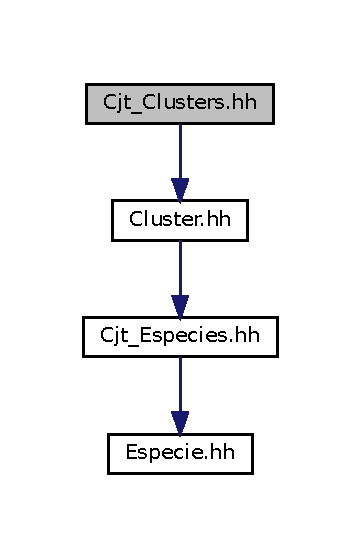
\includegraphics[width=256pt]{_cjt___clusters_8hh__incl}
\end{center}
\end{figure}
\subsection*{Classes}
\begin{DoxyCompactItemize}
\item 
class \hyperlink{class_cjt___clusters}{Cjt\+\_\+\+Clusters}
\begin{DoxyCompactList}\small\item\em Representa un conjunt de clusters. \end{DoxyCompactList}\end{DoxyCompactItemize}


\subsection{Descripció Detallada}
Especificació de la classe \hyperlink{class_cjt___clusters}{Cjt\+\_\+\+Clusters}. 


\hypertarget{_cjt___especies_8hh}{}\section{Referència del Fitxer Cjt\+\_\+\+Especies.\+hh}
\label{_cjt___especies_8hh}\index{Cjt\+\_\+\+Especies.\+hh@{Cjt\+\_\+\+Especies.\+hh}}


Especificació de la classe \hyperlink{class_cjt___especies}{Cjt\+\_\+\+Especies}.  


Inclou el graf de dependències per a Cjt\+\_\+\+Especies.\+hh\+:\nopagebreak
\begin{figure}[H]
\begin{center}
\leavevmode
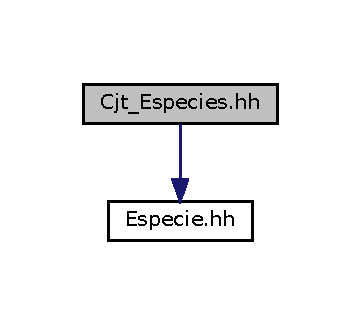
\includegraphics[width=173pt]{_cjt___especies_8hh__incl}
\end{center}
\end{figure}
\subsection*{Classes}
\begin{DoxyCompactItemize}
\item 
class \hyperlink{class_cjt___especies}{Cjt\+\_\+\+Especies}
\begin{DoxyCompactList}\small\item\em Representa un conjunt d\textquotesingle{}espècies. \end{DoxyCompactList}\end{DoxyCompactItemize}


\subsection{Descripció Detallada}
Especificació de la classe \hyperlink{class_cjt___especies}{Cjt\+\_\+\+Especies}. 


\hypertarget{_cluster_8hh}{}\section{Referència del Fitxer Cluster.\+hh}
\label{_cluster_8hh}\index{Cluster.\+hh@{Cluster.\+hh}}


Especificació de la classe \hyperlink{class_cluster}{Cluster}.  


Inclou el graf de dependències per a Cluster.\+hh\+:
\nopagebreak
\begin{figure}[H]
\begin{center}
\leavevmode
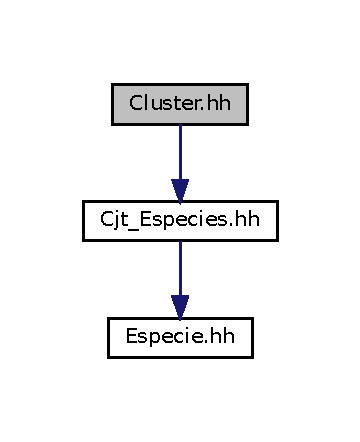
\includegraphics[width=173pt]{_cluster_8hh__incl}
\end{center}
\end{figure}
\subsection*{Classes}
\begin{DoxyCompactItemize}
\item 
class \hyperlink{class_cluster}{Cluster}
\begin{DoxyCompactList}\small\item\em Representa un cluster format per un idcluster i Bin\+Tree. \end{DoxyCompactList}\end{DoxyCompactItemize}


\subsection{Descripció Detallada}
Especificació de la classe \hyperlink{class_cluster}{Cluster}. 


\hypertarget{_especie_8hh}{}\section{Referència del Fitxer Especie.\+hh}
\label{_especie_8hh}\index{Especie.\+hh@{Especie.\+hh}}


Especificació de la classe \hyperlink{class_especie}{Especie}.  


\subsection*{Classes}
\begin{DoxyCompactItemize}
\item 
class \hyperlink{class_especie}{Especie}
\begin{DoxyCompactList}\small\item\em Representa una espècie amb un identificador i un gen. \end{DoxyCompactList}\end{DoxyCompactItemize}


\subsection{Descripció Detallada}
Especificació de la classe \hyperlink{class_especie}{Especie}. 


\hypertarget{program_8cc}{}\section{Referència del Fitxer program.\+cc}
\label{program_8cc}\index{program.\+cc@{program.\+cc}}


Programa principal de la pràctica.  


Inclou el graf de dependències per a program.\+cc\+:\nopagebreak
\begin{figure}[H]
\begin{center}
\leavevmode
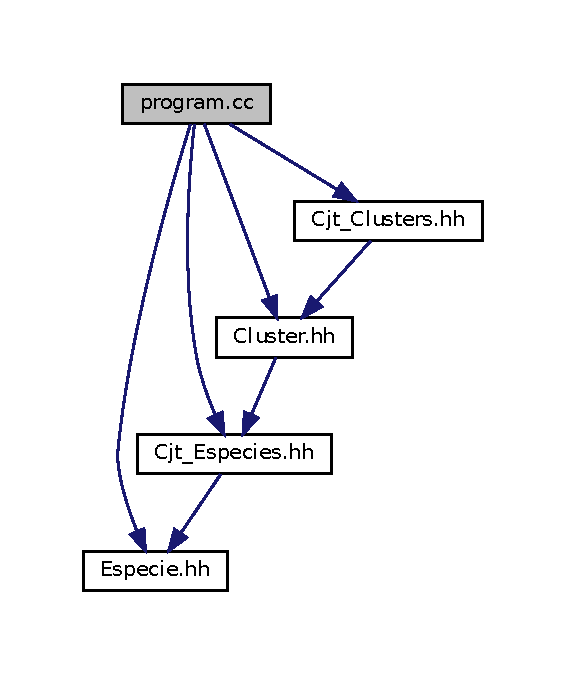
\includegraphics[width=256pt]{program_8cc__incl}
\end{center}
\end{figure}
\subsection*{Funcions}
\begin{DoxyCompactItemize}
\item 
int \hyperlink{program_8cc_ae66f6b31b5ad750f1fe042a706a4e3d4}{main} ()
\end{DoxyCompactItemize}


\subsection{Descripció Detallada}
Programa principal de la pràctica. 



\subsection{Documentació de les Funcions}
\mbox{\Hypertarget{program_8cc_ae66f6b31b5ad750f1fe042a706a4e3d4}\label{program_8cc_ae66f6b31b5ad750f1fe042a706a4e3d4}} 
\index{program.\+cc@{program.\+cc}!main@{main}}
\index{main@{main}!program.\+cc@{program.\+cc}}
\subsubsection{\texorpdfstring{main()}{main()}}
{\footnotesize\ttfamily int main (\begin{DoxyParamCaption}{ }\end{DoxyParamCaption})}



Definició a la línia 19 del fitxer program.\+cc.


\begin{DoxyCode}
19            \{
20     \textcolor{keywordtype}{int} k;
21     cin >> k;
22     \hyperlink{class_cjt___especies}{Cjt\_Especies} A;
23     \hyperlink{class_cjt___clusters}{Cjt\_Clusters} B;
24     \textcolor{keywordtype}{string} opcio;
25     \textcolor{keywordflow}{while} (cin >> opcio) \{
26         \textcolor{keywordflow}{if} (opcio == \textcolor{stringliteral}{"crea\_especie"}) \{
27             \textcolor{keywordtype}{string} id, g;
28             cin >> \textcolor{keywordtype}{id} >> g;
29             cout << \textcolor{stringliteral}{"# crea\_especie "} << \textcolor{keywordtype}{id} << \textcolor{stringliteral}{" "} << g << endl;
30             \textcolor{keywordflow}{if} (A.\hyperlink{class_cjt___especies_a2ce9d7a4968d46686109477f448857ea}{species\_exist}(\textcolor{keywordtype}{id})) \{
31                 cout << \textcolor{stringliteral}{"ERROR: La especie "}<< \textcolor{keywordtype}{id} << \textcolor{stringliteral}{" ya existe."} << endl;
32             \}
33             \textcolor{keywordflow}{else} \{
34                 \hyperlink{class_especie}{Especie} a(\textcolor{keywordtype}{id}, g, k);
35                 A.\hyperlink{class_cjt___especies_ab0aafd7fe0f24410a24aec9ff934bce0}{add\_species}(a);
36             \}
37             cout << endl;
38         \}
39         \textcolor{keywordflow}{else} \textcolor{keywordflow}{if} (opcio == \textcolor{stringliteral}{"obtener\_gen"}) \{
40             \textcolor{keywordtype}{string} id;
41             cin >> id;
42             cout << \textcolor{stringliteral}{"# obtener\_gen "} << \textcolor{keywordtype}{id} << endl;
43             \textcolor{keywordflow}{if} (A.\hyperlink{class_cjt___especies_a2ce9d7a4968d46686109477f448857ea}{species\_exist}(\textcolor{keywordtype}{id})) \{
44                 \hyperlink{class_especie}{Especie} a = A.\hyperlink{class_cjt___especies_a1e01bf8dfbde0983404efba05bd1b4b3}{find\_species}(\textcolor{keywordtype}{id});
45                 cout << a.\hyperlink{class_especie_a0781a594e45e036c0b59d161a7ebd8f3}{query\_gene}() << endl;
46             \}
47             \textcolor{keywordflow}{else} cout << \textcolor{stringliteral}{"ERROR: La especie "}<< \textcolor{keywordtype}{id} << \textcolor{stringliteral}{" no existe."} << endl;
48             cout << endl;
49         \}
50         \textcolor{keywordflow}{else} \textcolor{keywordflow}{if} (opcio == \textcolor{stringliteral}{"distancia"}) \{
51             \textcolor{keywordtype}{string} id1, id2;
52             cin >> id1 >> id2;
53             cout << \textcolor{stringliteral}{"# distancia "} << id1 << \textcolor{stringliteral}{" "} << id2 << endl;
54             \textcolor{keywordflow}{if} (not A.\hyperlink{class_cjt___especies_a2ce9d7a4968d46686109477f448857ea}{species\_exist}(id1) and not A.\hyperlink{class_cjt___especies_a2ce9d7a4968d46686109477f448857ea}{species\_exist}(id2)) cout << \textcolor{stringliteral}{"
      ERROR: La especie "} << id1 << \textcolor{stringliteral}{" y la especie "} << id2 << \textcolor{stringliteral}{" no existen."} << endl;
55             \textcolor{keywordflow}{else} \textcolor{keywordflow}{if} (not A.\hyperlink{class_cjt___especies_a2ce9d7a4968d46686109477f448857ea}{species\_exist}(id2)) cout << \textcolor{stringliteral}{"ERROR: La especie "} << id2 << \textcolor{stringliteral}{" no
       existe."} << endl;
56             \textcolor{keywordflow}{else} \textcolor{keywordflow}{if} (not A.\hyperlink{class_cjt___especies_a2ce9d7a4968d46686109477f448857ea}{species\_exist}(id1)) cout << \textcolor{stringliteral}{"ERROR: La especie "} << id1 << \textcolor{stringliteral}{" no
       existe."} << endl;
57             \textcolor{keywordflow}{else} cout << A.\hyperlink{class_cjt___especies_abf55093b325fd101ef73aa18dd1cf823}{species\_distance}(id1, id2) << endl;
58             cout << endl;
59 
60         \} 
61         \textcolor{keywordflow}{else} \textcolor{keywordflow}{if} (opcio == \textcolor{stringliteral}{"elimina\_especie"}) \{
62             \textcolor{keywordtype}{string} id;
63             cin >> id;
64             cout << \textcolor{stringliteral}{"# elimina\_especie "} << \textcolor{keywordtype}{id} << endl;
65             \textcolor{keywordflow}{if} (A.\hyperlink{class_cjt___especies_a2ce9d7a4968d46686109477f448857ea}{species\_exist}(\textcolor{keywordtype}{id})) \{
66                 A.\hyperlink{class_cjt___especies_ad72a47e0a785ac34f4908b54dd413d32}{erase\_species}(\textcolor{keywordtype}{id});
67             \} \textcolor{keywordflow}{else} cout << \textcolor{stringliteral}{"ERROR: La especie "} << \textcolor{keywordtype}{id} << \textcolor{stringliteral}{" no existe."} << endl;
68 
69             cout << endl;
70         \}
71         \textcolor{keywordflow}{else} \textcolor{keywordflow}{if} (opcio == \textcolor{stringliteral}{"existe\_especie"}) \{
72             \textcolor{keywordtype}{string} id;
73             cin >> id;
74             cout << \textcolor{stringliteral}{"# existe\_especie "} << \textcolor{keywordtype}{id} << endl;
75             \textcolor{keywordflow}{if} (A.\hyperlink{class_cjt___especies_a2ce9d7a4968d46686109477f448857ea}{species\_exist}(\textcolor{keywordtype}{id})) cout << \textcolor{stringliteral}{"SI"} << endl;
76             \textcolor{keywordflow}{else} cout << \textcolor{stringliteral}{"NO"} << endl;
77             cout << endl;
78         \} 
79         \textcolor{keywordflow}{else} \textcolor{keywordflow}{if} (opcio == \textcolor{stringliteral}{"lee\_cjt\_especies"}) \{
80             \textcolor{keywordtype}{int} n;
81             cin >> n;
82             A.\hyperlink{class_cjt___especies_a273156c50e67be8815bdd1c31cc1661a}{read\_species}(n, k);
83             cout << \textcolor{stringliteral}{"# lee\_cjt\_especies"} << endl;
84             cout << endl;
85             
86         \}
87         \textcolor{keywordflow}{else} \textcolor{keywordflow}{if} (opcio == \textcolor{stringliteral}{"imprime\_cjt\_especies"}) \{ \textcolor{comment}{//falta buidar}
88             cout << \textcolor{stringliteral}{"# imprime\_cjt\_especies"} << endl;
89             A.\hyperlink{class_cjt___especies_a362d2295d52e2a4cb3618bda7ad3f65b}{print\_species}();
90             cout << endl;
91         \}
92         \textcolor{keywordflow}{else} \textcolor{keywordflow}{if} (opcio == \textcolor{stringliteral}{"tabla\_distancias"}) \{
93             cout << \textcolor{stringliteral}{"# tabla\_distancias"} << endl;
94             A.\hyperlink{class_cjt___especies_ab6ebf81bf6ad734a970c3677fd4e5250}{print\_table\_species}();
95             cout << endl;
96         \}
97         \textcolor{keywordflow}{else} \textcolor{keywordflow}{if} (opcio == \textcolor{stringliteral}{"inicializa\_clusters"}) \{
98             cout << \textcolor{stringliteral}{"# inicializa\_clusters"} << endl;
99             B.\hyperlink{class_cjt___clusters_a35d2c4c28bee51017f4ac9049a0fe6e9}{initialize\_clusters}(A);
100             B.\hyperlink{class_cjt___clusters_acc4dd33e82c36c394acd44e60f77da22}{print\_table\_clusters}();
101             cout << endl;
102         \}
103 
104         \textcolor{keywordflow}{else} \textcolor{keywordflow}{if} (opcio == \textcolor{stringliteral}{"ejecuta\_paso\_wpgma"}) \{
105             cout << \textcolor{stringliteral}{"# ejecuta\_paso\_wpgma"} << endl;
106             \textcolor{keywordflow}{if} (B.\hyperlink{class_cjt___clusters_a1ecfc9a82c3a0dff467769880c355efd}{clusters\_set\_size}() > 1) \{
107                 B.\hyperlink{class_cjt___clusters_ac2bf2811c291533e3516ad4de8240d36}{wpgma\_algorithm}();
108                 B.\hyperlink{class_cjt___clusters_acc4dd33e82c36c394acd44e60f77da22}{print\_table\_clusters}();
109             \} \textcolor{keywordflow}{else} cout << \textcolor{stringliteral}{"ERROR: num\_clusters <= 1"} << endl;
110             cout << endl;
111         \}
112         \textcolor{keywordflow}{else} \textcolor{keywordflow}{if} (opcio == \textcolor{stringliteral}{"imprime\_cluster"}) \{
113             \textcolor{keywordtype}{string} id;
114             cin >> id;
115             cout << \textcolor{stringliteral}{"# imprime\_cluster "} << \textcolor{keywordtype}{id} << endl;
116             \textcolor{keywordflow}{if} (B.\hyperlink{class_cjt___clusters_aaa57cbd8d86567b4403ac9adb34a87f5}{cluster\_exist}(\textcolor{keywordtype}{id})) \{
117                 \hyperlink{class_cluster}{Cluster} aux = B.\hyperlink{class_cjt___clusters_a4ab91d8e8222f35b4c9592c5ab2b4bf3}{find\_cluster}(\textcolor{keywordtype}{id});
118                 B.\hyperlink{class_cjt___clusters_aa9a896c44d86f130747f1e6821a4dddd}{print\_cluster}(aux);
119                 cout << endl;
120             \} \textcolor{keywordflow}{else} cout << \textcolor{stringliteral}{"ERROR: El cluster "} << \textcolor{keywordtype}{id} << \textcolor{stringliteral}{" no existe."} << endl;
121             cout << endl;
122         \}
123         \textcolor{keywordflow}{else} \textcolor{keywordflow}{if} (opcio == \textcolor{stringliteral}{"imprime\_arbol\_filogenetico"}) \{
124             cout << \textcolor{stringliteral}{"# imprime\_arbol\_filogenetico"} << endl;
125             B.\hyperlink{class_cjt___clusters_a35d2c4c28bee51017f4ac9049a0fe6e9}{initialize\_clusters}(A);
126             \textcolor{keywordflow}{if} (B.\hyperlink{class_cjt___clusters_a1ecfc9a82c3a0dff467769880c355efd}{clusters\_set\_size}() < 1) cout << \textcolor{stringliteral}{"ERROR: El conjunto de clusters es
       vacio."} << endl;
127             \textcolor{keywordflow}{else} \{
128                 \textcolor{keywordflow}{while} (B.\hyperlink{class_cjt___clusters_a1ecfc9a82c3a0dff467769880c355efd}{clusters\_set\_size}() > 1) \{
129                     B.\hyperlink{class_cjt___clusters_ac2bf2811c291533e3516ad4de8240d36}{wpgma\_algorithm}();
130                 \}
131                 \hyperlink{class_cluster}{Cluster} aux = B.\hyperlink{class_cjt___clusters_a48cb7ca0417ba1de9593a00f98d91880}{query\_final\_cluster}();
132                 B.\hyperlink{class_cjt___clusters_aa9a896c44d86f130747f1e6821a4dddd}{print\_cluster}(aux);
133                 
134 
135                 cout << endl;
136             \}
137             cout << endl;
138         \}
139         \textcolor{keywordflow}{else} \textcolor{keywordflow}{if} (opcio == \textcolor{stringliteral}{"fin"}) \{
140             \textcolor{keywordflow}{break};
141         \}
142     \}
143 
144 
145 \}
\end{DoxyCode}

%--- End generated contents ---

% Index
\backmatter
\newpage
\phantomsection
\clearemptydoublepage
\addcontentsline{toc}{chapter}{Índex}
\printindex

\end{document}
